\let\accentvec\vec
\documentclass[]{llncs}
\usepackage{colortbl}
\usepackage{silence}
\WarningFilter{todonotes}{The length}
\WarningFilter{caption}{Unsupported}
\WarningFilter{caption}{Forced redefinition}
\WarningFilter{caption}{The option}
\WarningFilter{caption}{Unknown document}

\let\spvec\vec
\let\vec\accentvec
\usepackage{amsmath}
\let\vec\spvec

\usepackage{url}
\usepackage{hyperref}
\usepackage{array}

\usepackage{caption}
%\usepackage[position=t]{subcaption}
\captionsetup{compatibility=false}
\usepackage{subcaption}
%\usepackage[caption=false]{subfig}

\usepackage{array}
\usepackage{cite}
\usepackage{amsmath,amssymb,amsfonts}
\usepackage{algorithmic}
\usepackage{graphicx}
\newsavebox{\imagebox}
\usepackage{textcomp}
\usepackage{xcolor}
\usepackage{listings}
\usepackage{lstautogobble}
\usepackage[listings,skins,breakable,raster,most]{tcolorbox}
\usepackage{numprint}
\usepackage{tikz}
\usetikzlibrary{positioning,shapes,arrows,fit,backgrounds}
\usepackage{booktabs}
\usepackage{multirow}
\usepackage{soul}
\usepackage{tabularx}
\usepackage{mathtools}

\usepackage{cleveref}
\crefname{codecount}{Code}{Codes}

\usepackage{todonotes}
\newcommand{\jk}[1]{\todo[inline]{JK:\@#1}}
\newcommand{\eb}[1]{\todo[inline]{EB:\@#1}}

\definecolor{tabhcolor}{rgb}{0.63, 0.79, 0.95}
\newcolumntype{$}{>{\global\let\currentrowstyle\relax}}
\newcolumntype{^}{>{\currentrowstyle}}
\newcommand{\rowstyle}[1]{\gdef\currentrowstyle{#1}%
	  #1\ignorespaces
	}




\usepackage{graphicx}
\graphicspath{%
	{./pictures/}
}

\lstset{%
	numberbychapter=false,
	belowskip=-10pt,
	aboveskip=10pt,
}

\lstdefinestyle{lstcodebox}{%
	basicstyle=\scriptsize\ttfamily,
	autogobble=true,
	tabsize=2,
	captionpos=b,
	float,
}

\renewcommand{\ttdefault}{pcr}
\lstdefinestyle{instylebf}{%
	basicstyle=\bfseries\scriptsize\ttfamily,
}

\lstdefinestyle{instyle}{%
	basicstyle=\scriptsize\ttfamily,
}

\lstdefinestyle{lstcommon}{ %
%\lstdefinestyle{sig}{ %
  %backgroundcolor=\color{white},   % choose the background color; you must add \usepackage{color} or \usepackage{xcolor}; should come as last argument
  basicstyle=\fontsize{8}{8}\ttfamily,        % the size of the fonts that are used for the code
  breakatwhitespace=false,         % sets if automatic breaks should only happen at whitespace
  breaklines=true,                 % sets automatic line breaking
  captionpos=n,                    % sets the caption-position to bottom
  %commentstyle=\color{mygreen},    % comment style
  deletekeywords={...},            % if you want to delete keywords from the given language
  %escapeinside={\%*}{*)},          % if you want to add LaTeX within your code
  extendedchars=true,              % lets you use non-ASCII characters; for 8-bits encodings only, does not work with UTF-8
  frame=none,                    % adds a frame around the code
  keepspaces=true,                 % keeps spaces in text, useful for keeping indentation of code (possibly needs columns=flexible)
  keywordstyle=\bf\ttfamily,       % keyword style
  language=C,                 % the language of the code
  morekeywords={*,...},           % if you want to add more keywords to the set
  %numbers=left,                    % where to put the line-numbers; possible values are (none, left, right)
  numbersep=5pt,                   % how far the line-numbers are from the code
  %numberstyle=\tiny\color{mygray}, % the style that is used for the line-numbers
  rulecolor=\color{black},         % if not set, the frame-color may be changed on line-breaks within not-black text (e.g. comments (green here))
  showspaces=false,                % show spaces everywhere adding particular underscores; it overrides 'showstringspaces'
  showstringspaces=false,          % underline spaces within strings only
  showtabs=false,                  % show tabs within strings adding particular underscores
  stepnumber=1,                    % the step between two line-numbers. If it's 1, each line will be numbered
  %stringstyle=\color{mymauve},     % string literal style
  tabsize=2,                    % sets default tabsize to 2 spaces
  title=\lstname                   % show the filename of files included with \lstinputlisting; also try caption instead of title
}


\lstset{ %
  autogobble=true,
  backgroundcolor=\color{white},   % choose the background color; you must add \usepackage{color} or \usepackage{xcolor}
  basicstyle=\scriptsize\ttfamily,       % the size of the fonts that are used for the code
  breakatwhitespace=false,         % sets if automatic breaks should only happen at whitespace
  breaklines=true,                 % sets automatic line breaking
  captionpos=b,                    % sets the caption-position to bottom
  %commentstyle=\color{green},    % comment style
  deletekeywords={...},            % if you want to delete keywords from the given language
  escapeinside={(*}{*)},          % if you want to add LaTeX within your code
  extendedchars=true,              % lets you use non-ASCII characters; for 8-bits encodings only, does not work with UTF-8
  frame=none,                    % (none, single) adds a frame around the code
  keepspaces=true,                 % keeps spaces in text, useful for keeping indentation of code (possibly needs columns=flexible)
  keywordstyle=\color{blue},       % keyword style
  language=Octave,                 % the language of the code
  otherkeywords={*,...},           % if you want to add more keywords to the set
  %numbers=left,                    % where to put the line-numbers; possible values are (none, left, right)
  numbersep=5pt,                   % how far the line-numbers are from the code
  numberstyle=\tiny\color{gray}, % the style that is used for the line-numbers
  rulecolor=\color{black},         % if not set, the frame-color may be changed on line-breaks within not-black text (e.g. comments (green here))
  showspaces=false,                % show spaces everywhere adding particular underscores; it overrides 'showstringspaces'
  showstringspaces=false,          % underline spaces within strings only
  showtabs=false,                  % show tabs within strings adding particular underscores
  stepnumber=1,                    % the step between two line-numbers. If it's 1, each line will be numbered
  stringstyle=\color{blue},     % string literal style
  tabsize=2,                     % sets default tabsize to 2 spaces
  title=\lstname,                  % show the filename of files included with \lstinputlisting; also try caption instead of title
}


\begin{document}

\title{Classifying Temporal Characteristics of Job I/O Patterns Using Machine Learning Techniques}


\institute{%
DKRZ -- \email{betke@dkrz.de}%
\and University of Reading--%
\email{j.m.kunkel@reading.ac.uk}%
}

\author{Eugen Betke \inst{1} \and  Julian Kunkel\inst{2}}

\maketitle

\begin{abstract}
Every day, supercomputers execute 1000s of jobs with different characteristics.
Data centers monitor the behavior of jobs to support the users and improve the infrastructure, for instance, by optimizing jobs or by determining guidelines for the next procurement.
The classification of jobs into groups that express similar run-time behavior aids this analysis as it reduces the number of representative jobs to look into.
This work utilizes machine learning techniques to cluster and classify parallel jobs based on the similarity in their temporal I/O behavior.
Our contribution is the qualitative and quantitative evaluation of different I/O characterizations and similarity measurements and the development of a suitable clustering algorithm.

In the evaluation, we explore I/O characteristics from monitoring data of one million parallel jobs and cluster them into groups of similar jobs.
Therefore, the time series of various IO statistics is converted into features using different similarity metrics that customize the classification.

When using general-purpose clustering techniques, suboptimal results are obtained.
Additionally, we extract phases of IO activity from jobs.
Finally, we simplify the grouping algorithm in favor of performance.
We discuss the impact of these changes on the clustering quality.
\end{abstract}

\textbf{Keywords: }IO fingerprinting, performance analysis, monitoring

\section{Introduction}
Scientific large-scale applications of different domains have different needs for I/O and, thus, exhibit a variety of access patterns on storage.
Even re-running the same simulation may lead to different behavior.
We can distinguish between a temporal behavior, i.e., the operations performed over time such as long read/write phases, bursty I/O pattern, and concurrent metadata operations, and spatial access pattern of individual processes of the application as they can be, e.g., sequential or random.

On different supercomputers, the same I/O patterns may result in different application runtimes depending on the nature of the access pattern.

For example, machines equipped with burst buffers \cite{10.1007/978-3-030-02465-9_9, 7004215} may significantly reduce application runtimes by absorbing bursty I/O traffic.
I/O congestion and file system performance degradation can occur when several I/O intensive jobs are running on the same machine at the same time.
I/O aware schedulers, like CARS~\cite{LIANG201925} and Flux~\cite{flux}, implement new scheduling strategies that utilize I/O metrics.
The analysis of I/O is important not only when I/O begins to take a considerable amount of application runtime but when I/O patterns begin to degrade the performance of the shared file system affecting runtimes of other applications and worsening user experience by unresponsive file systems~\cite{10.1007/978-3-030-02465-9_5}.

Understanding the exhibited I/O behavior and implications on the system would give users and administrators information to support analysis by revealing deficiencies and may indicate the potential for I/O optimization.
Knowing the potential for optimization is important for the support staff, as it allows them to identify applications that benefit from I/O optimizations.
For example, a widely used parallel application that still utilizes sequential I/O might be cost-efficient to optimize.

The main question is how to identify such applications automatically from the observed data.
Non-intrusive capturing of I/O metrics and the analysis can be challenging in many aspects.
Firstly, in order to find optimization potential, data must be recorded in an appropriate level of detail to retain temporal characteristics.
While capturing statistics on node level is supported by many monitoring tools, e.g., LASSi~\cite{sivalingam2019lassi}, Darshan\cite{hpcdarshan}, and SIOX\cite{TSACAMAOOP14}.
Detailed metrics on file level are more difficult to obtain.
A widespread method is re-implementation and pre-loading of an I/O interface, which contains monitoring code.

However, recording the data isn't enough, the obtained data must be processed but the manual analysis is infeasible as the number of jobs is large -- Monitoring systems of HPC systems record data of ten thousand jobs each day.
Hence a semi-automatic approach is required to reduce the number of jobs to investigate.

In a previous paper, we proposed a semi-automatic way to find relevant jobs by computing relevant job characteristics from time series of job behavior.
Basically, support staff could then focus on those IO-intense jobs that express certain metrics the most.
Here, we extend the approach by grouping similar jobs based on profiles and IO-phases in order to simplify the investigation effort.

In different disciplines, machine learning methods have proven to be powerful tools to extract new information from large data sets.
Therefore, we explore clustering strategies on monitoring data, to reveal hidden information.

This paper is organized as follows: Section 2 outlines the preliminary work and provides background knowledge that is important to understand the next sections.
In Section 3, we discuss the key problem we are dealing with.
In Section 4, we introduce\ alternative approaches for the clustering, as different goals for the analysis require different distance metrics, we discuss the variety of approaches.
We start with a simple solution and increase complexity.
The results and discussion are attached to the methodology of each solution as subsections.
Finally, in Section 5 we summarize the results.


\section{Preliminary Work}
The German Climate Computing Center (DKRZ) maintains a monitoring system that gathers various statistics from the Mistral HPC system.
Mistral has 3,340 compute nodes, 24 login nodes, and two Lustre file systems (lustre01 and lustre02) that provide a capacity of 52 Petabyte.
The monitoring system is made up of open source components such as Grafana, OpenTSDB, and Elasticsearch but also includes a lightweight self-developed data collector that captures continuously node statistics - we decided to implement an own collector when analyzing the overhead of existing approaches.
Additionally, the monitoring system obtains various job meta-information from the Slurm workload manager and injects selected log files.

Our motivation for automatic analysis of parallel jobs is the monitoring situation at DKRZ.
Mistral runs around 10.000 jobs a day, which is too much for manual analysis.
In our previous work~\cite{iocats2020}, we found a way to identify I/O intensive jobs and jobs with inefficient usage by deriving statistics from the node-level statistics.
This information can aid the procurement of new HPC systems or support the extension of an existing one.
While this approach helps to find individual jobs, it doesn't provide a global overview, which might be more important for making decisions at the data center perspective.
For example, a discovery of a large group of I/O-intensive and bursty applications would suggest attaching a burst buffer to the storage, to improve application runtimes.
In this paper, we take up the idea of I/O categorization from the previous work, where we partition job runtime into equal size segments and map them into three categories (LowIO, HighIO, and CriticalIO), and continue our work to obtain a global overview.

A difference to previously utilized job statistics is that this time Lustre proc files on Mistral doesn't offer Object Storage Client (osc) counters, since a major upgrade of Lustre file system from version 2.7 to 2.11.
Thus, instead of 13 metrics, this time our data contains only 9 metrics.

Understanding of the following work requires an understanding of data format, that is formed by segmentation and categorization of raw monitoring data.
Segmentation is a pre-processing step that splits data into equal-sized segments and computes a mean performance for each segment.
This stage preserves the performance units (e.g., Op/s, MiB/s) for each metric.
As further calculations that involve different metrics is difficult for different metrics, we introduced a categorization\textbf{ pre-processing} step that takes into account the performance of the underlying HPC system and assigns an ordered category to each segment.
It takes the mean performance that was calculated in the previous step, and assigns one of the three categories (LowIO=0, HighIO=1 and CriticalIO=4).
The category split points are based on the histogram of the obtained values, for any metrics, a segment with a value up to the 99\%-Quantile it is considered to be LowIO, the 99.9\%-Quantile indicates HighIO~(see \cite{iocats2020}).
This node-level data can then be used to compute job-statistics by aggregating across time, file systems, and nodes.

In summary, this data representation has the following key advantages for data analysis.
The ordered categories make the calculations between different metrics feasible, which is not possible with raw data.
Furthermore, the domains are equally scaled and compatible, because the values are between 0 and 4, and a value has a meaning.
Besides, the resulting data representation is much smaller compared to the raw data.
This allows us to apply compute-intensive algorithms to large datasets.
Finally, irrelevant data is hidden by the LowIO category and doesn't distract from significant parts of jobs.

In our previous work, we computed three high-level metrics per job that aid users to understand job profiles:

\begin{itemize}
	\item \textbf{Job-I/O-Balance:} indicates how I/O load is distributed between nodes during job runtime.
	\item \textbf{Job-I/O-Utilization:} shows the average I/O load during I/O-phases.
	\item \textbf{Job-I/O-Problem-Time} is the fraction of job runtime that is I/O-intensive; it is approximated by the fractions of segments that are considered I/O intensive.
\end{itemize}

\begin{figure}[!bt]
	\centering
	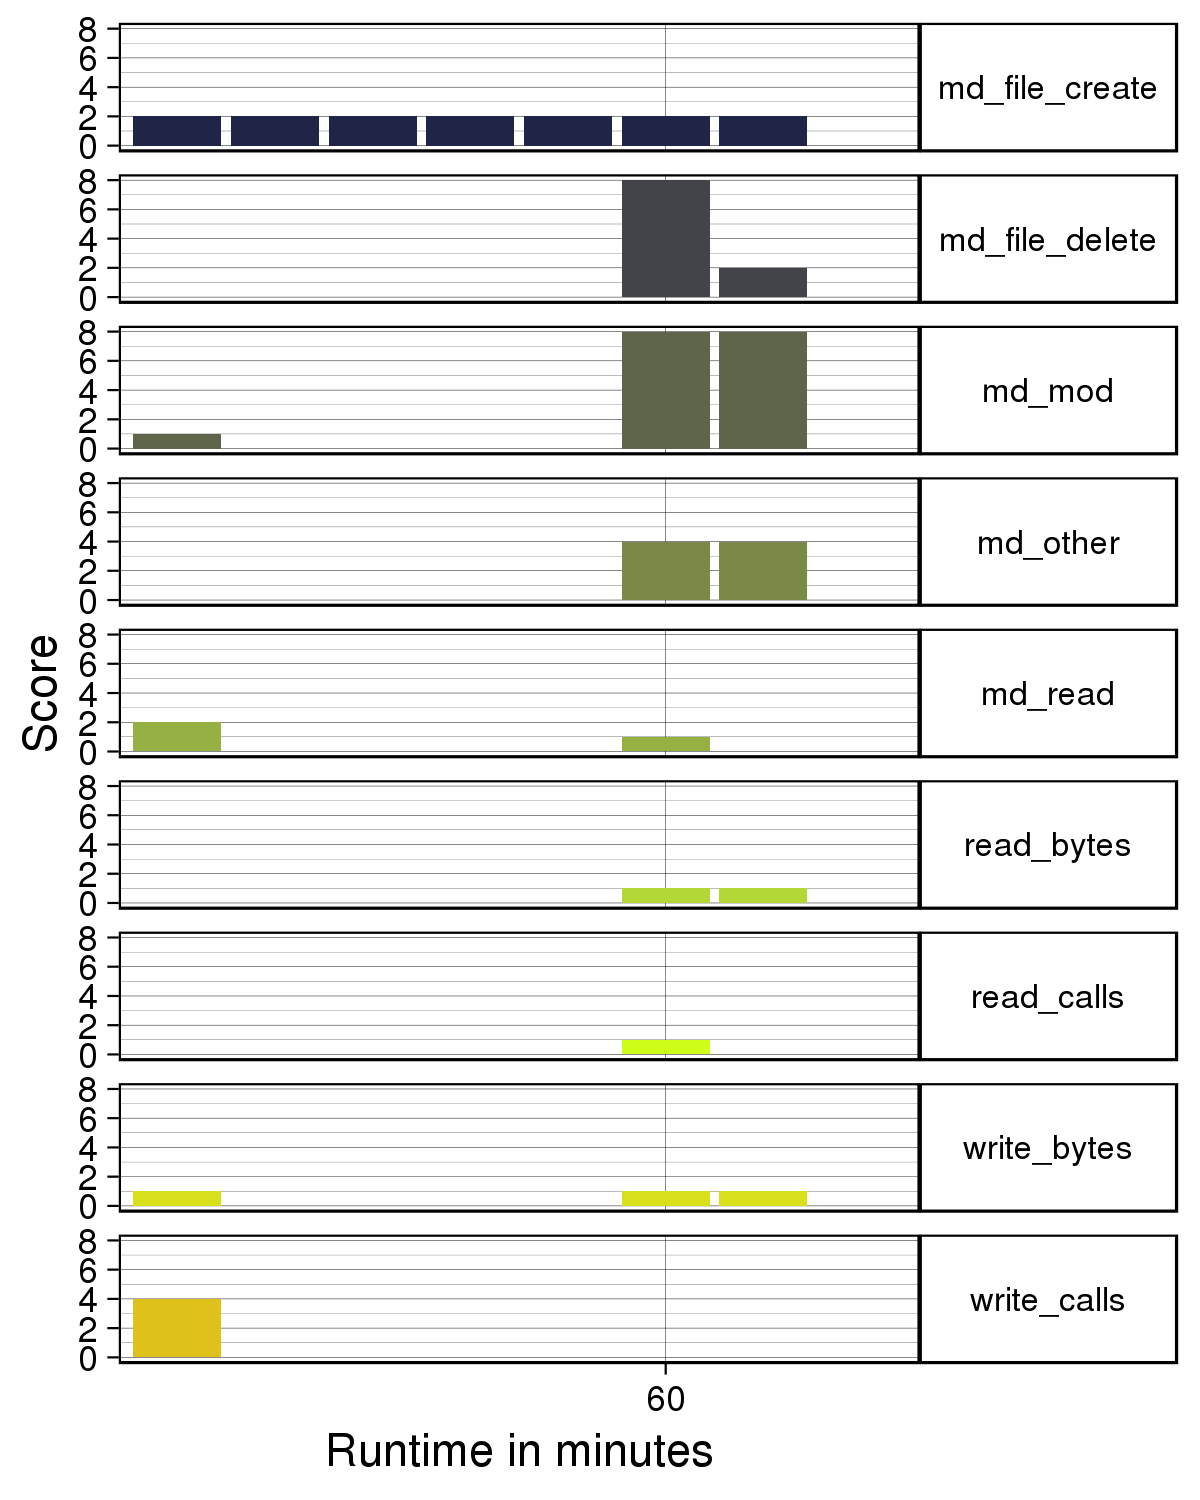
\includegraphics[width=2.02in,height=2.52in]{./media/image4.png}
	\caption{Example job-level metric. Score is the sum of all node scores.}
	\label{fig:seg_example}
\end{figure}

In \Cref{fig:seg_example}, we can see the temporal behavior for this particular job when summing up the node-level metrics.
We call \textbf{an I/O phase a contiguous sequence of non-zero segments} (where the score of the segment is larger than zero).
For example, in the figure, we can see one phase for md\_file\_create, and two phases for md\_mod (one short and non-intrusive at the beginning, and one critical around 60 minutes).

When looking at categorization at the metric level, i.e., after reduction of the nodes and file system dimensions, we can observe that many jobs exhibit I/O phases.

\section{Similarity Between Jobs}
The raw monitoring data of a job in our environment at DKRZ, we obtain a time series of 9 metrics per node, each metrics sampled at five seconds intervals.
When comparing the time series of such metrics between two jobs, the key question is how do we define the similarity between multiple time series.
By applying dimensionality reduction techniques such as PCR, we can reduce the complexity and potentially obtain a similar representation for, e.g., two time series, but cannot make relevant distinctions between them.

First, we need to discuss the similarity of IO patterns from the user perspective.
In \Cref{fig:typ_io:all}, we illustrate the time series of two metrics for three different jobs.
The figures show the typical behavior of parallel applications, computation is interrupted by regular I/O phases -- by phase, we mean a consecutive segment of time in which  certain behavior is exhibited, i.e., the statistics are similarly.

Actually,\ the shape of I/O phases depends on our definition of I/O phase.
By applying dimension reduction techniques, I/O phases from different dimensions can be joined together.
Although several different aggregations are possible, in this work we focus on  I/O phases on metrics, i.e, we aggregate nodes and file system dimensions.
Identification of I/O phases shows that a substantial number of jobs has several of them.

From the user support side, we might be interested in grouping similar suboptimal jobs and aim to provide one recipe to optimize all that exhibit such a behavior.
Similarly, we might be interested to optimize the pattern for a single I/O phase.
We may be interested to ignore computation time and focus on I/O phases only.
Regardless of the segment of the time series we look at, we naively would consider an IO pattern to be identical if the time series for all metrics of one job is identical to those of another job.
Unfortunately, the obtained measurements vary due to the nature of parallel applications and the environment of the data center they are executed.
In practice, different jobs show a different runtime, and even when re-running the same job, the obtained time series varies.

\begin{figure}
        \centering
         \begin{subfigure}[t]{\textwidth}
           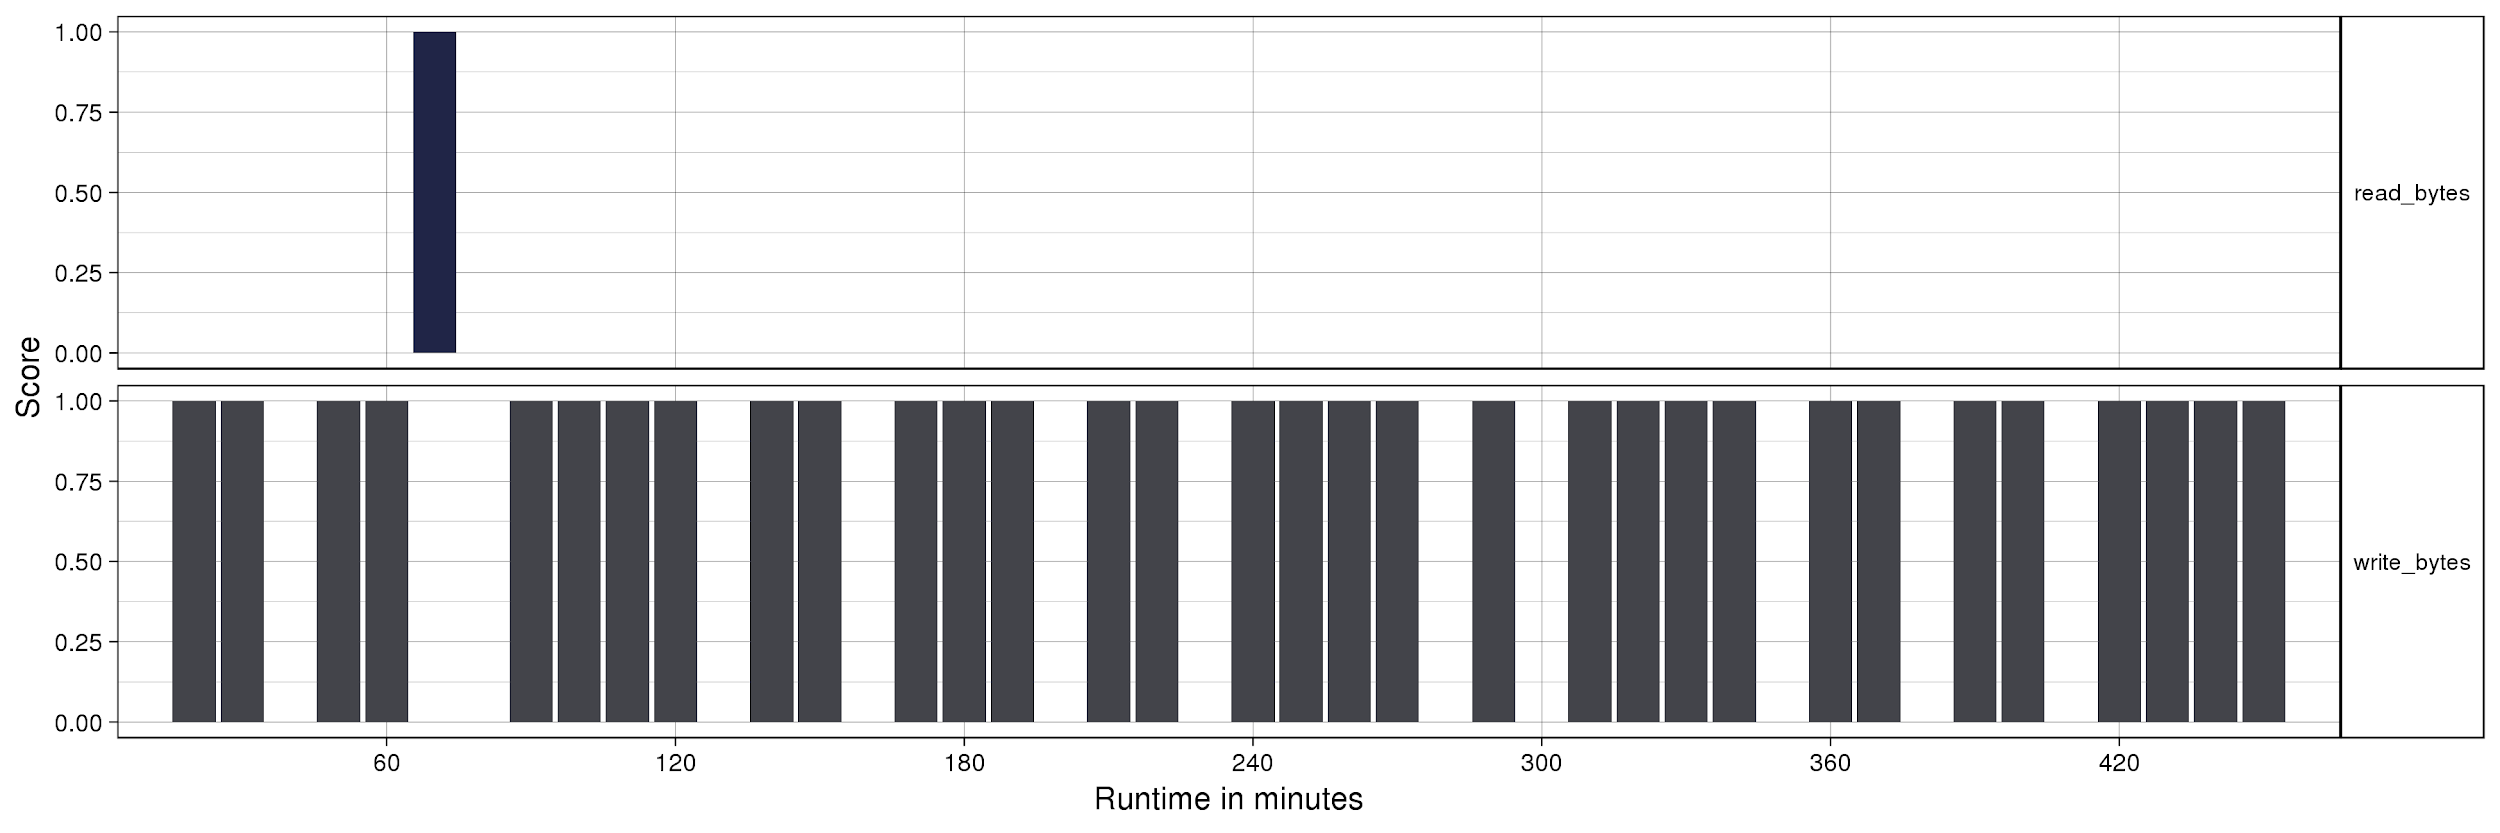
\includegraphics[width=4.61in,height=1.54in]{./media/image27.png}
           \caption{Job A runs on 13 nodes}
           \label{fig:typ_io:1}
         \end{subfigure}

        \begin{subfigure}[t]{\textwidth}
           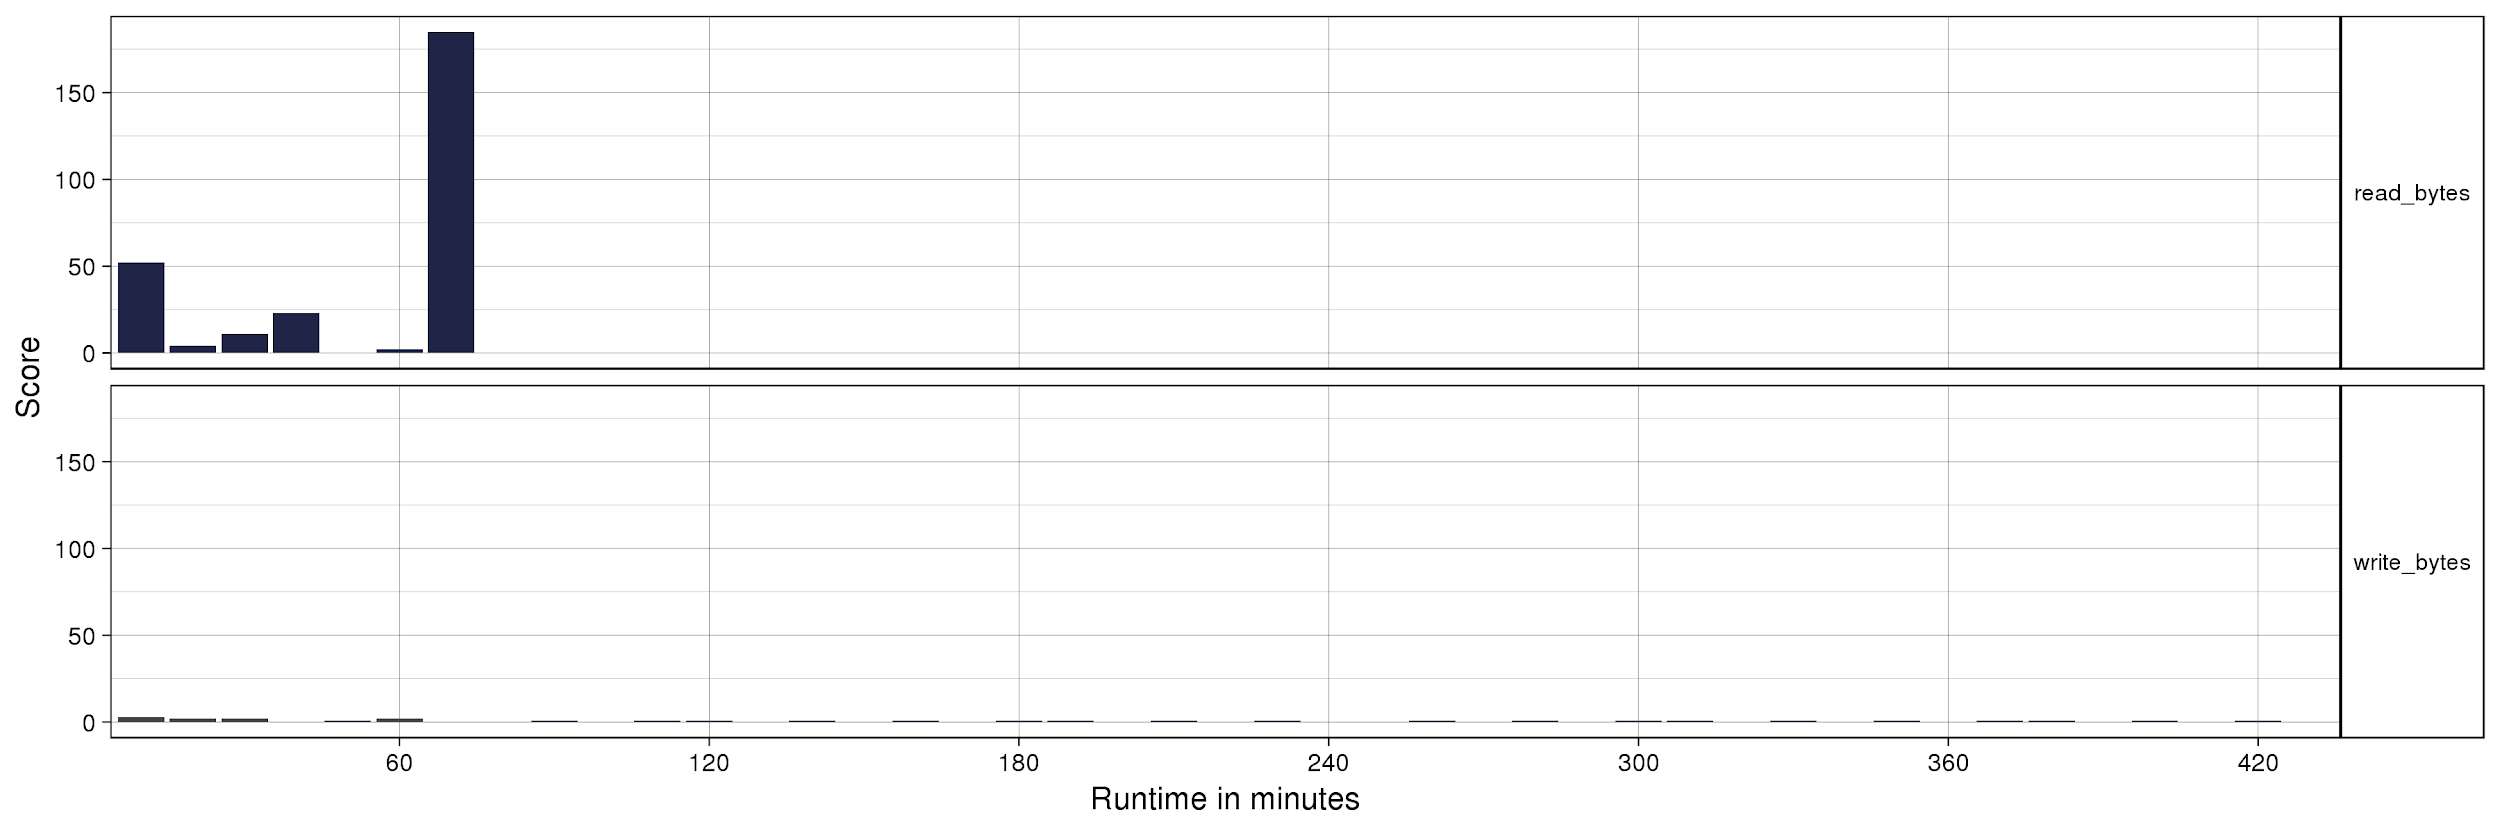
\includegraphics[width=4.61in,height=1.54in]{./media/image28.png}
           \caption{Job B runs on 225 nodes}
           \label{fig:typ_io:2}
         \end{subfigure}

        \begin{subfigure}[t]{\textwidth}
          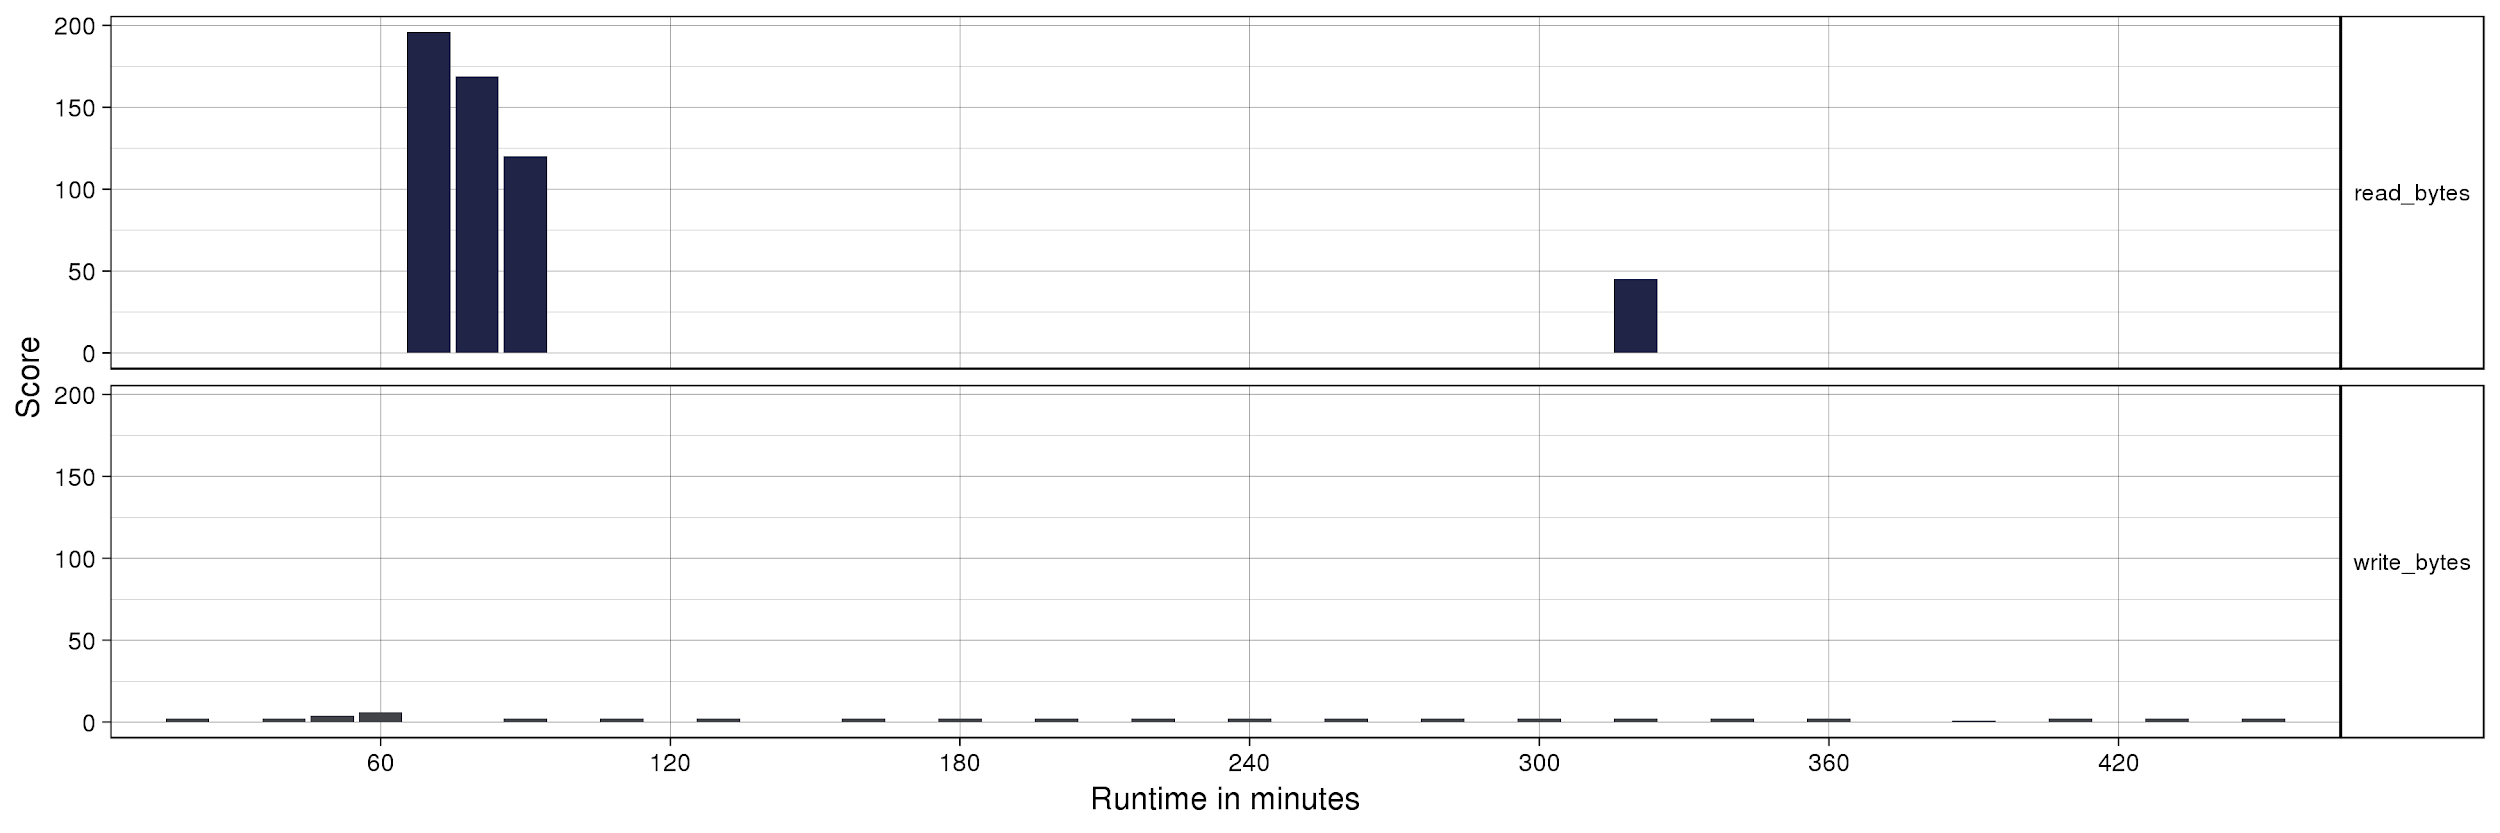
\includegraphics[width=4.61in,height=1.54in]{./media/image25.png}
          \caption{Job C runs on 40 nodes}
          \label{fig:typ_io:3}
        \end{subfigure}
\caption{Monitoring data of three jobs. Score is the sum of individual node scores.}
         \label{fig:typ_io:all}
\end{figure}

Typical sources of variability when observing performance metrics are: The concurrent usage of the shared storage, a shift between observed I/O phases due to network congestion or CPU throttling for power/heat reasons.
The same application using a different input configuration may need more compute time, resulting in longer phases between typical I/O patterns; moreover, it may change the I/O pattern.
A well-known pattern exhibited by a shorter running application may appear as well in a long-running application.
The similarity measure between two jobs should consider those sources of variability and allow us to provide a robust clustering of jobs depending on the user question.

There are different goals for the data analysis done by the user running the application or the support staff of the data center.
Whether or not the timeline is similar when executing an application with a different configuration and input dataset depends on the purpose of the analysis and task that follows the analysis.
For these reasons, we decided to explore a variety of alternative options for distance metrics and pre-processing and assess their suitability.


\section{Related work}
There are many tracing and profiling tools that are able to record I/O information~\cite{TFAPIKBBCF19}; we will discuss a selection of them in more detail in the following.Most of them focus on individual jobs, and only a few of them apply machine learning for data analysis, in particular across jobs.As the purpose of applications is computation and, thus, I/O is just a byproduct, applications often spend less than 10\% time with I/O.The issue of performance profiles is that they remove the temporal dimension and make it difficult to identify relevant I/O phases.The Ellexus tools\footnote{\url{https://www.ellexus.com/products/}} include Breeze, a user-friendly offline I/O profiling software, an automatic I/O report generator Healthcheck, and command line tool Mistral which purpose is to report on and resolve I/O performance issues when running complex Linux applications on high performance compute clusters.Mistral is a small program that allows you to monitor application I/O patterns in real time, and log undesirable behaviour using rules defined in a configuration file called a contract.
Darshan~\cite{carns2011understanding-toc,hpcdarshan} is an open source I/O characterization tool for post-mortem analysis of HPC applications' I/O behavior.Its primary objective is to capture concise but useful information with minimal overhead.Darshan accomplishes this by eschewing end-to-end tracing in favor of compact statistics such as elapsed time, access sizes, access patterns, and file names for each file opened by an application.These statistics are captured in a bounded amount of memory per process as the application executes.When the application shuts down, it is reduced, compressed, and stored in a unified log file.%Utilities included with Darshan can then be used to analyze, visualize, and summarize the Darshan log information.Because of Darshan's low overhead, it is suitable for system-wide deployment on large-scale systems.In this deployment model, Darshan can be used not just to investigate the I/O behavior of individual applications but also to capture a broad view of system workloads for use by facility operators and I/O researchers.

There are approaches that monitor record storage behavior and aim to identify inefficient applications in a cluster.
TOKIO~\cite{lockwood2018tokio} integrates logs from various sources to allow an analysis of data.
It allows finding certain inefficient access patterns in the data.
The LASSi tool~\cite{DBLP:journals/corr/abs-1906-03884} was developed for detecting, the so called, victim and aggressor applications.An aggressor can steal I/O resources from the victim and negatively affect its runtime.To identify such applications, LASSi calculates metrics from Lustre job-stats and information from the job scheduler.One metric category shows file system load and another category describes applications I/O behavior.The correlation of these metrics can help to identify applications that cause the file system to slow down.In the LASSi workflow this is a manual step, where a support team is involved in the identification of applications during file system slow down.Manual steps are disadvantageous when processing large amounts of data and must be avoided in unsupervised I/O behavior identification.LASSi's indicates that the main target group are system maintainers.Understanding LASSi reports may be challenging for ordinary HPC users, who do not have knowledge about the underlying storage system.

In~\cite{TUISVPKB19}, the authors utilized probes to detect file system slow-down.A probing tool measures file system response times by periodically sending metadata and read/write requests.An increase of response times correlates to the overloading of the file system.This approach allows the calculation of a slow-down factor identification of the slow-down time period.This approach is able to detect a file system slow-down, but cannot detect the jobs that cause the slow-down.
The Nextgenio monitoring system~\cite{nextgenio2016}, has four main collectors.The first two, the PBS and ALPS tools, collect job scheduling information.The proprietary Cray I/O monitoring tool exploits Lustre I/O counters to capture file system usage on OSTs of all OSSs and allocated compute nodes.The MAP component provides information about cpu, memory and network usage.Then all the collected data is clustered for the analysis of system usage and performance evaluation.In contrast to existing approaches, our approach focuses on the analysis of job data and investigates clustering strategy to group similar jobs.

\section{Methodology}

The goal of this article is to research the impact of clustering strategies on a large number of jobs. Generally, machine learning algorithms expect a fixed number of features, therefore, the time series of statistics that is retrieved on the node-level needs to be pre-processed.
The application of a “specific algorithm” can be understood as a number of successive processing steps on data. Roughly speaking, there are three basic steps: data pre-processing including coding, similarity computation, and clustering.
We call one of such a combination a \textit{clustering stack}.
The pre-processing converts the dynamic-sized monitoring data which depends on the number of captured metrics, allocated nodes, and application runtime into a suitable representation for the clustering algorithm.
Then the clustering is applied. Finally, the clustering result needs to be assessed, i.e., how suitable is this strategy for our IO statistics and use cases?

In the following, we have dedicated a section to each step listing and briefly discussing potential alternatives.
The list does not intend to be complete but shows a variety of options.

\subsubsection{Data pre-processing}
The 4-dimensional data from our monitoring system is too fine-grained for mass analysis,
to be able to analyze millions of jobs, we must apply some data reduction technique.
The result of the data-preprocessing is a coding of the initial time series data into one or multiple vectors.

We first convert the time series into segments of 10 minutes which we found previously is a good trade-off to represent the temporal behavior of the application while it reduces the size of the time series.
Hence, for a job and for each of our 9 client-side recorded metrics, we obtain a coarse-grained time series.
To simplify the interpretation of results and the choice distance metrics, it is beneficial to have the same unit for all features which is why we use our category classification which creates a unitless order.
For example, when reduced by node, file system, and across metrics, a point may represent the mean value across all time series for the job for the 10 minute interval.

On the high-level, the following strategies for data reduction could be considered:
\begin{itemize}
	\item \textbf{Job profiles} compute statistics across the whole job by eliminating the temporal component by applying reduction operations such as the arithmetic mean.
		A drawback of this simplification is that any temporal pattern is lost.
	\item \textbf{Segment statistics} compute for each segment a fixed statistics, such as the mean value across all nodes.
		This basically preserves the time series and depends on the job-length.
	\item \textbf{Phase statistics} computes high-level statistics by analyzing the temporal behavior of IO phases further, e.g., compute the average length of IO segments with CriticalIO.
		This approach is independent of the job length but requires identifying phases and determining meaningful job metrics.
\end{itemize}

We decided to distinguish the different dimensions of a job (Node, File System, Metric, and Time) defining how the aggregation is performed.
Not reducing data in the dimension would mean that the result would depend on e.g., the number of nodes of a job, which makes the analysis difficult.
For one dimension, you could compute various statistics, we decided to use mean or sum.
Any data reduction is performed in this order: fist Node, File System, and last by Metric, thus, a time series of encoded segments remain.
The time series of segments can be reduced differently in each dimension; alternatives that we apply in this paper are listed in \Cref{tab:reduction_techniques}.
By reducing along all dimension, you obtain basically a job profile (as discussed above).

\begin{table}
	\centering
	\begin{tabularx}{\textwidth}{llX}
		Dimension       & Operation                                    &  Description                                                       \\
		\hline
		Node            & Reduce by mean()                             &  Aggregate all nodes by mean() function                            \\
		                & Reduce by sum()                              &  Aggregate all nodes by sum() function                             \\
		\hline
		File System     & Reduce by mean()                             &  Aggregate all file systems by mean() function                     \\
		                &
		Reduce by sum() & Aggregate all file systems by sum() function \\
		\hline
		Metric          & Reduce by sum()                              &  Aggregate all nine metrics by sum()                               \\
		\hline
		Time            &                                              &  Convert segments to coding formats \\
		\hline
    All     & Reduce by mean()    &  Reduces time series to a fixed set of values                      \\
		\hline
	\end{tabularx}
	\caption{Dimension reduction strategies for the original 4D-data.}
	\label{tab:reduction_techniques}
\end{table}

\subsubsection{Coding}

Segmented data contains a numeric floating point value for each data, which can be too much information for the analysis.
Therefore, we introduce two condensed data representations called binary and hexadecimal coding.
Additionally, we introduce two operations on the coding:
the first extracts I/O phases -- a phase is a consecutive non-zero series of segments;
the second merges all consecutive zero segments into one segment, i.e., removes compute phases in the statistics.
The operations are summarized in \Cref{tab:coding_ops}.

\begin{table}
 \centering
 \begin{tabularx}{\textwidth}{lX}
	 Operation &  Description \\
	 \hline	 Binarization & Segments are mapped to 9-bit numbers (v), where each position (i) represents a metric. The bits are set by the following function:
	 \vbox{
		\begin{equation}
			v_i =
			\begin{cases}
				\text{false if segment}_i = 0\\\text{true otherwise.}
			\end{cases}, i \in [\text{enumerated metrics}]
		\end{equation}
	 } \\
	 \hline
	 Hex-Quantization & Quantize segments to 16 levels. \\
	 \hline
	 Zeros aggregation & Merge all consecutive zero segments. \\
	 \hline
	 Phase extraction &  Extract continuous sequences of non-zero segments. \par - Split time series at zero segments in sub time series (I/O phases) and remove zero segments. \par - Preserve order of I/O phases. \\
	 \hline
 \end{tabularx}
 \caption{Coding operations.}
 \label{tab:coding_ops}
\end{table}
\paragraph{Binary coding}
Binary coding represents monitoring data as a sequence of numbers, where each number represents the overall file system usage.
The number is computed based on the 9 metrics found in the segment, e.g., if a phase is read and write intensive it is encoded as one type of behavior.
In this approach, each conceivable combination of activities has an unique number.

The approach maps the three categories to the following two states: The LowIO category is mapped to the non-active (0) state, and HighIO and CriticalIO categories are mapped to the active (1) state.
On one side, by doing this, we lose information about performance intensity, but on other side, this simplification allows a more comprehensible comparison of job activities.

In our implementation, we use a 9-bit number to represent each segment, where each bit represents a metric.
The bit is 1 if the corresponding metric is active, and 0 if not.
Translated to the decimal representation, metric segments can be coded as 1, 2, 4, 8, 16, and so on.
Using this kind of coding we can compute a number for each segment, that describes unambiguously the file system usage, e.g., a situation where intensive usage of md\_read (Code=16) and read\_bytes (Code=32) occur at the same time and no other significant loads are registered is coded by the value 48.
Coding is reversible, e.g., when having value 48, the computation of active metrics is straightforward.

%\begin{table}[H]
%       \centering
%\begin{tabular}{p{0.8in}p{0.8in}}
%\hline
%%row no:1
%\multicolumn{1}{p{0.8in}}{\cellcolor[HTML]{C9DAF8} \tabto{0.25in}  \tabto{0.39in} \tab Metric} &
%\multicolumn{1}{p{0.8in}}{\cellcolor[HTML]{C9DAF8} \tabto{0.25in}  \tabto{0.39in} \tab Code} \\
%\hhline{--}
%%row no:2
%\multicolumn{1}{p{0.8in}}{md\_file\_create} &
%\multicolumn{1}{p{0.8in}}{ \tabto{0.25in}  \tabto{0.39in} \tab 1} \\
%\hhline{~~}
%%row no:3
%\multicolumn{1}{p{0.8in}}{md\_file\_delete} &
%\multicolumn{1}{p{0.8in}}{ \tabto{0.25in}  \tabto{0.39in} \tab 2} \\
%\hhline{~~}
%%row no:4
%\multicolumn{1}{p{0.8in}}{md\_mod} &
%\multicolumn{1}{p{0.8in}}{ \tabto{0.25in}  \tabto{0.39in} \tab 4} \\
%\hhline{~~}
%%row no:5
%\multicolumn{1}{p{0.8in}}{md\_other} &
%\multicolumn{1}{p{0.8in}}{ \tabto{0.25in}  \tabto{0.39in} \tab 8} \\
%\hhline{~~}
%%row no:6
%\multicolumn{1}{p{0.8in}}{md\_read} &
%\multicolumn{1}{p{0.8in}}{ \tabto{0.25in}  \tabto{0.39in} \tab 16} \\
%\hhline{~~}
%%row no:7
%\multicolumn{1}{p{0.8in}}{read\_bytes} &
%\multicolumn{1}{p{0.8in}}{ \tabto{0.25in}  \tabto{0.39in} \tab 32} \\
%\hhline{~~}
%%row no:8
%\multicolumn{1}{p{0.8in}}{read\_calls} &
%\multicolumn{1}{p{0.8in}}{ \tabto{0.25in}  \tabto{0.39in} \tab 64} \\
%\hhline{~~}
%%row no:9%\multicolumn{1}{p{0.8in}}{write\_bytes} &%\multicolumn{1}{p{0.8in}}{ \tabto{0.25in}  \tabto{0.39in} \tab 128} \\
%\hhline{~~}
%%row no:10
%\multicolumn{1}{p{0.8in}}{write\_calls} &
%\multicolumn{1}{p{0.8in}}{ \tabto{0.25in}  \tabto{0.39in} \tab 256} \\
%\hhline{~~}
%\end{tabular}
% \end{table}

To reduce the 4-dimensional data, we reduce that structure to two dimensions (segments metrics) by aggregating other dimensions by applying sum() function on score values.
In the resulting table we leave zero scores, and change scores larger than zero to one.
After coding each segment, the jobs can be represented as a sequence of numbers, e.g.,
\begin{lstlisting}
'jobid': 'jobA', 'coding': [1:5:0:0:0:0:0:0:96:96:96:96:96:96:96], 'length': 15
\end{lstlisting}
The monitoring dataset doesn't provide information about what happens during the zero segments.
It can be anything, like a job is waiting for resources, or computing something.
It can also be that the job script cannot start immediately or run on a slow network.
To catch such jobs, we aggregate multiple consecutive zero segments into one zero segment, thus the coding of the previous job would replace all 0:...:0 sequences just with 0.

\begin{lstlisting}
'jobid': 'jobA', 'coding': [1:5:0:96:96:96:96:96:96:96], 'length': 15
\end{lstlisting}

Note, that the job length does not change, only the sequence length.

\paragraph*{Hexadecimal coding}

This coding preserves monitoring data for each metric and each segment.
As the name suggests, the value of a segment is converted into a hexadecimal number to allow creation of a string representing the IO behavior.
The numbers are obtained in two steps.
Firstly, the dimension reduction aggregates the file system and the node dimensions and computes a mean value for each metric and segment, which lies in the interval [0,4].
Secondly, the mean values are quantized into 16 levels -- 0 represents the interval [0,0.125), 1 [0.125,0.375), $ \ldots $ , [3.625,4].
The example in \Cref{tab:hex_example} shows hexadecimal coding for a job containing 6 segments.

\begin{table}
  \centering
  \begin{tabular}{ll}
    md\_file\_create & [00\textbf{2}\textbf{2}\textbf{2}\textbf{9}] \\
    md\_file\_delete & [000000]                                     \\
    md\_mod          & [000000]                                     \\
    md\_other        & [000000]                                     \\
    md\_read         & [000\textbf{9}30]                            \\
    read\_bytes      & [\textbf{5}00000]                            \\
    read\_calls      & [000000]                                     \\
    write\_bytes     & [0000\textbf{f}\textbf{f}]                   \\
    write\_calls     & [000000]
  \end{tabular}
  \caption{Example of a hexadecimal coding for 6 segments.}
  \label{tab:hex_example}
\end{table}

\subsubsection{Similarity}
Determining the resemblance between two jobs is the main task of this work.
Clustering algorithms need a distance metrics to allow organizing them together.
There are various variants, a selection is listed in \Cref{tab:sim_funcs}.
The Manhatten distance for two vectors is defines as $\sum_i |a_i - b_i|$ and can naturally only be applied to vectors of the same length.
The Levensthein distance is the number of modifications (inserts, deletes, changes) of individual characters that need to be made to transform one string to another.
To create a flexible similarity function, we combine the Manhatten distance with a sliding window or phase detection to allow it to determine a distance between two vectors of different length.

\begin{table}
  \centering
  \begin{tabularx}{\textwidth}{lX}
    Distance & Description \\
    \hline
    Manhatten & The Manhatten distance between the vectors. \\
    \hline
    Levenshtein &  Number of operation (inserts, deletes, and changes) requires to convert one coding in another \\
    \hline
    \hline
    \multicolumn{2}{l}{Options for Manhatten} \\
    \hline
    Sliding window &  - Find maximum similarity between two codings \par
            - Slide shorter coding over a longer one an compute similarity of the corresponding parts \\
    \hline
    Phase &  - Find best I/O phases combination of two jobs with a maximum similarity \par - Depends on phase extraction from data pre-processing and sliding window similarity \par - Preserve the order of the phases \\
    \hline
  \end{tabularx}
  \caption{Similarity functions and strategies}
  \label{tab:sim_funcs}
\end{table}

\subsubsection{Clustering}
In the last step, similar jobs need to be grouped in clusters.
A subset of potential strategies is listed in \Cref{tab:clustering_algorithms}.
Often, the k-means algorithm is applied which utilizes a random strategy to initialize clusters.
However, as it requires us to define a fixed number of clusters, it is problematic as the number of actual clusters are unknown.
The large class of density clustering algorithms such as DBSCAN groups objects that are "close" together into one class; a user defines the maximum distance of objects that belong to the same class by setting an $\epsilon$ which represents the similarity value.
Agglomerative strategies group similar elements together to form a hierarchy of some sort, e.g., a tree.
Unfortunately, their complexity is quadratic at least.
To handle millions of jobs, an algorithm must be performant.

We developed two strategies that address the performance issue and the other limitations, the ClusteringTree algorithm and the SimplifiedDensity algorithm.
These algorithms are able to handle the large number of jobs but aim to preserve the core ideas of k-means/density algorithms.
They are described in the following:

\begin{table}
  \centering
  \begin{tabularx}{\textwidth}{lX}
    Algorithm & Description \\
    \hline
    k-means & Runs a random initialization, then refines the clusters until the clusters don't change any more. \\
    \hline
    Density clustering &  Group nearby elements recursively together as long as they are ($\epsilon$) close together. \\
    \hline
    Agglomerative &  Hierarchically cluster data into groups of elements that belong closer together. \\
    \hline
    \textbf{ClusteringTree} &  Create a hierarchical clustering for subset of data to train a decision tree, then apply the decision tree on the full dataset. \\
    \hline
    \textbf{SimplifiedDensity} &  Combines ideas from k-means with density clustering. The simplified clustering algorithms add a job to a cluster if similarity to the cluster centroid is equal or larger than the user defined value. \\
    \hline
  \end{tabularx}
  \caption{Selection of clustering algorithms}
  \label{tab:clustering_algorithms}
\end{table}
\paragraph{ClusteringTree algorithm}
This algorithm involves three steps:

\begin{enumerate}
 \item Agglomerative clustering of a small dataset, enumerate leaf-level clusters that are similar.
 \item Training of a decision tree model on the small dataset, i.e., the tree should decide in which cluster a job is stored.
 \item Clustering of the large data set using the decision tree.
\end{enumerate}

Since the number of clusters on leaf-level depends on their similarity, this strategy should determine a number of suitable clusters that mimics the job distribution in the training set.

\paragraph{SimplifiedDensity algorithm}

The algorithm forms clusters around centroids.
These are job codings that form clusters by attracting similar jobs.
All jobs in a cluster fulfill only one condition, the similarity (SIM) to the centroid has to be bigger than the user defined minimum, in that sense it is similar to DBSCAN.
It is approximative as the order of jobs matters for the creation of the clusters.

The algorithm can be summarized as follows:
\begin{enumerate}
 \item Pick one arbitrary job from the dataset, which will serve as a cluster centroid, and compute similarity to all other jobs.
 \item Create a cluster of jobs that have a minimum similarity and remove them from the dataset.
 \item Repeat step 1 and 2 until no jobs are left in the dataset.
\end{enumerate}

This approach allows a performant implementation, but they also allow a job to be in one cluster, even if a centroid of another cluster is much closer, as long as the condition is true.
Hence, the result depends on the processing order of the jobs, though it is deterministic.


\subsubsection{Clustering stacks}
There are various combinations possible of the different strategies.

\begin{figure}
  \centering
  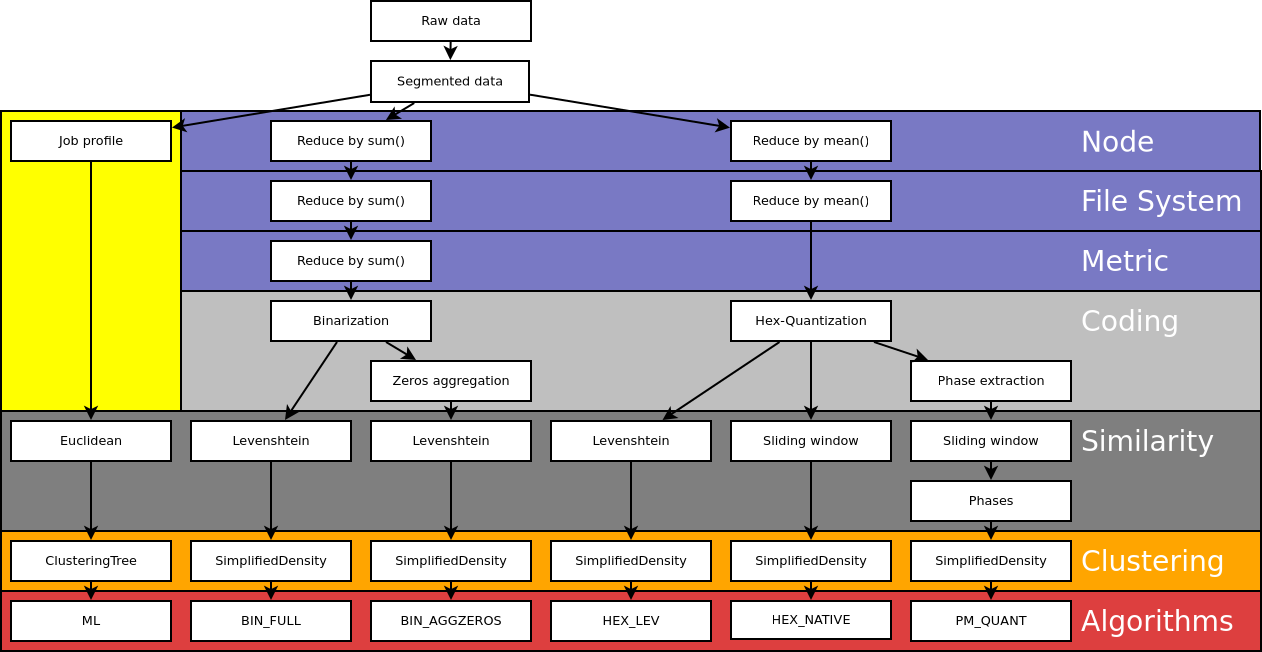
\includegraphics[width=4.61in,height=2.38in]{./media/image3.png}
  \caption{Algorithms and their actual operation stacks.}
  \label{fig:clustering_stacks}
\end{figure}

For simplicity, we refer to one clustering stack just as algorithm.
During our research, we explored various combinations out of the possible combinations but we found that these do not perform well and are not interesting to discuss.

The operation stack which we describe in this article is visualized in \Cref{fig:clustering_stacks}.
In brief, the algorithms are as follows:
\begin{itemize}
 \item (ML) uses a set of \textbf{traditional machine learning} techniques on job profiles.
 \item (BIN\_ALL) uses \textbf{Levenshtein} distance on \textbf{binary codings.}
 \item (BIN\_AGGZEROS) is like BIN\_ALL, but with \textbf{zero aggregation} of contiguous zero segments.
 \item (HEX\_LEV) uses \textbf{hexadecimal coding} and \textbf{Levenshtein} distance.
 \item (HEX\_NATIVE) is like HEX\_LEV, but uses a \textbf{performance-aware} similarity function.
 \item (PM\_QUANT) is like HEX\_NATIVE, but uses a \textbf{phase-aware} similarity function.
\end{itemize}

\subsection{Algorithms}
This section describes the evaluated algorithms in detail.

\subsubsection{ML}

To apply existing clustering algorithms, first, a job-profile is created in the pre-processing.
The 4d time series can be transformed into the required fixed size input format accepted by the general-purpose ML clustering algorithms.
We explored two job profiles: IO-metric and I/O-duration.
The \textbf{IO-metric job profile} utilizes three features, Job-I/O-Balance, Job-I/O-Utilization, and Job-I/O-Problem-Time (as defined in \cite{iocats2020}).
After the data pre-processing, we obtain a set of 3-dimensional data points with a domain between 0 and 1.
The maximum distance between any two jobs ($SIM_{max}$) is 1.44.

The \textbf{IO-duration job profile} contains the fraction of runtime, a job spent doing the individual I/O categories leading to 27 columns.
The columns are named according to the following scheme: metric\_category, e.g, bytes\_read\_0 or md\_file\_delete\_4.
The first part is the one of the nine metric names and the second part is the category number (LowIO=0, HighIO=1 and CriticalIO=4).
These columns are used for machine learning as input features.
There is a constraint for each metric (metric\_0 + metric\_1 + metric\_4 = 1), that makes 9 features redundant, because they can be computed from the other features.
So we have to deal with 18 features; $SIM_{max}$ is 1.17.

\jk{Warum ist das hier 1.17, checke ich nicht}

\paragraph{Clustering algorithm}
We intended to apply agglomerative clustering.
\jk{Könnte noch bissl unklar sein}
The algorithm uses Euclidean distance as a similarity measure, i.e., if the component wise distance between two job vectors is shorter than the defined distance (SIM), then these jobs belong to the same cluster.

We found that the size of our datasets is the first obstacle to the suitable clustering algorithms.
For example, the scaling behavior of the agglomerative clustering algorithm that is used in this work can handle around 10,000 jobs in a reasonable amount of time as the complexity is \(N^{2}\).

Therefore, to be able to cluster 1,000,000 samples, we created a variant of the algorithm by utilizing a decision tree.
This workaround involves three steps:

\begin{enumerate}
 \item Cluster and label 10,000 jobs with the agglomerative clustering algorithm
 \item Train a decision tree model with data from the previous step
 \item Predict labels of 1,000,000 jobs with the trained decision tree model
\end{enumerate}

\subsubsection{BIN\_ALL}
This algorithm converts the time series data via binary coding to a string and then determine the relative similarity using the Levenshtein distance.

The Levenshtein based similarity between two jobs is determined using \Cref{eq:lev}.
\begin{equation}
similarity \left( job_{A}\text{, jo}b_{B} \right) =1- \frac{levenshtein \left( coding_{A}\text{, codin}g_{B} \right) }{max \left( length_{A}\text{, lengt}h_{B} \right) } \label{eq:lev}
\end{equation}
It is the number of Levenshtein operations (changes/deletes/inserts) divided by the length of the longest sequence, and subtracted from the value one.

\begin{lstlisting}
'jobid': 'jobA', 'coding': [1:5:0:0:0:0:0:0:96:96:96:96:96:96:96], 'length': 15
'jobid': 'jobB', 'coding': [0:0:0:0:0:0:0:0:0:96:96:96:96:96:98], 'length': 15
\end{lstlisting}

The similarity between these two jobs is 73 percent.

\subsubsection{BIN\_AGGZEROS}
This is a variant of BIN\_ALL where subsequent zero-sequences are reduced to a single zero segment before \Cref{eq:lev} is applied.
This allows us to focus on I/O intensive parts of the job.
The example below shows the reduced codings from the previous example.
\begin{equation}
similarity \left( job_{A}\text{, jo}b_{B} \right) =1- \frac{levenshtein \left( coding_{A}\text{, codin}g_{B} \right) }{max \left( length_{A}\text{, lengt}h_{B} \right) }
\end{equation}

The two previous jobs are now encoded slightly different leading to a similarity of 53 percent:
\begin{lstlisting}
'jobid': 'jobA', 'coding': [1:5:0:96:96:96:96:96:96:96], 'length': 15
'jobid': 'jobB', 'coding': [0:96:96:96:96:96:98], 'length': 15
\end{lstlisting}

\subsubsection{HEX\_LEV}
This algorithm works on the same principle like the BIN algorithms, with the difference that it applies a hexadecimal coding and then computes the mean similarity across all metrics using Levenshtein.
This adaption allows a comparison of time series where one metrics differs as only one metric string would differ while with binary coding the overall string would be different.

\begin{multline}
  similarity \left( job_{A}\text{, jo}b_{B} \right) = 1 -\frac{ \sum_{m \in Metrics}^{} levenshtein \left( coding_{A,m}\text{, coding}_{B,m} \right) }{|Metrics| \cdot L_{B}} \\
	\text{with } L_{B} \geq L_{A}
\end{multline}

\subsubsection{HEX\_NATIVE}
This algorithm computes a performance-aware similarity between two jobs.
It works with hexadecimal codings at metric level and basically computes the relative similarity using the Manhatten distance.
Assume jobB is larger or equal than jobA, the job similarity between two jobs can be computed using \Cref{eq:hexn}.

\begin{multline}
similarity \left( job_{A}\text{, jo}b_{B} \right) = 1-\frac{ \sum _{m \in Metric}^{}maxSimilarity \left( job_{A,m}\text{, jo}b_{B,m} \right) }{L_{B}}\\
\text{with }L_{B} \geq L_{A} \label{eq:hexn}
\end{multline}

The metric coding sequences $job_{B,m}$ and $job_{A,m}$ of different jobs can have different lengths.
Therefore, to compute a maximum similarity between two metrics, we use a sliding window approach.
That means, we take the shortest coding sequence (CA) and check how it fits best on the longer coding sequence (CB).


\begin{lstlisting}
float maxSimilarity(CA, CB) {
  max = 0
  LA = length(CA)
  LB = length(CB)
  for pos in 0..(LB-LA) { // LB-LA is the boundary, as stated: LB > LA
    sim = sliceSimilarity(CA, substr(str=CB, start=pos, len=LA))
    if sim > max {
      max = sim
    }
  }
  return max
}
\end{lstlisting}

The \texttt{sliceSimilarity()} in \Cref{eq:slicesim} function computes similarity between two codings of the same length.
This function maps the difference between performance levels of the same segments (values between 0 and 16) to a relative value between 0 and 1.

\begin{equation}
sliceSimilarity \left( S_{A},S_{B} \right) =\frac{ \sum _{i=1}^{L_{}}16 - \vert S_{A,i}-S_{B,i} \vert }{\text{16 L}_{}}\text{, with }L=L_{B}=L_{A} \label{eq:slicesim}
\end{equation}

\subsubsection{PM\_QUANT}
The phase-matching quantization algorithm allows us to cluster variable length words.
First, using a hexadecimal coding, phases of consecutive I/O segments are detected and extracted.
Then, the best match between the (disjoint) phases is determined, finally the similarity is computed.

We will discuss the details of each step on the following example; a blue font emphasizes I/O intensive  metrics.

\begin{lstlisting}[language=C,morekeywords={md_file_create,read_bytes}]
jobA (length: 13)
md_file_create [0:0:2:2:2:9:3:0:9:1:1:1:0]
md_file_delete [0:0:0:0:0:0:0:0:0:0:0:0:0]
md_mod         [0:0:0:0:0:0:0:0:0:0:0:0:0]
md_other       [0:0:0:0:0:0:0:0:0:0:0:0:0]
md_read        [0:0:0:0:0:0:0:0:0:0:0:0:0]
read_bytes     [0:0:0:9:3:0:0:0:0:0:1:0:0]
read_calls     [0:0:0:0:0:0:0:0:0:0:0:0:0]
write_bytes    [0:0:0:0:0:0:0:0:0:0:0:0:0]
write_calls    [0:0:0:0:0:0:0:0:0:0:0:0:0]
\end{lstlisting}

\vspace*{-0.5em}

\begin{lstlisting}[language=C,morekeywords={md_file_create,read_bytes,write_bytes}]
jobB (length: 15)
md_file_create [1:0:0:0:0:0:0:0:0:0:0:0:0:0:0]
md_file_delete [0:0:0:0:0:0:0:0:0:0:0:0:0:0:0]
md_mod         [0:0:0:0:0:0:0:0:0:0:0:0:0:0:0]
md_other       [0:0:0:0:0:0:0:0:0:0:0:0:0:0:0]
md_read        [0:0:0:0:0:0:0:0:0:0:0:0:0:0:0]
read_bytes     [2:2:2:2:8:2:2:0:0:1:0:0:8:1:1]
read_calls     [0:0:0:0:0:0:0:0:0:0:0:0:0:0:0]
write_bytes    [0:0:0:0:0:0:0:0:0:0:0:5:0:0:0]
write_calls    [0:0:0:0:0:0:0:0:0:0:0:0:0:0:0]
\end{lstlisting}

\paragraph{Phase detection}
According to our I/O phase definition, phases are separated by zeros.
This definition makes the detection of individual phases to a trivial task.
Relevant for similarity computation are only metrics that contain at least one non-zero segment.
In this example, that is md\_file\_create, read\_bytes and write\_bytes metrics:
\begin{lstlisting}
job_A_md_file_create : [[2,2,2,9,3], [9,1,1,1]]
job_A_read_bytes : [[9,3], [1]]
job_A_write_bytes : []

job_B_md_file_create : [[1]]
job_B_read_bytes : [[2,2,2,2,8,2,2], [1], [8,1,1]]
job_B_write_bytes : [[5]]
\end{lstlisting}

\paragraph{Phase matching}
Now we slide the shorter phase over the longer and compute similarity to the corresponding part such that we can find the best match.
In the example, the best match is found on position five.

\noindent\begin{minipage}{0.33\textwidth}
\begin{lstlisting}
[2:2:2:2:8:2:2]
[9:3:-:-:-:-:-]
similarity
= (2/9+2/3)/7
= 13%

[2:2:2:2:8:2:2]
[-:9:3:-:-:-:-]
similarity
= (2/9+2/3)/7
= 13%
\end{lstlisting}
\end{minipage}
%
\noindent\begin{minipage}{0.33\textwidth}
\begin{lstlisting}
[2:2:2:2:8:2:2]
[-:-:9:3:-:-:-]
similarity
= (2/9+2/3)/7
= 13%

[2:2:2:2:8:2:2]
[-:-:-:9:3:-:-]
similarity
= (2/9+3/8)/7
= 8%
\end{lstlisting}
\end{minipage}
%
\noindent\begin{minipage}{0.33\textwidth}
\begin{lstlisting}
[2:2:2:2:8:2:2]
[-:-:-:-:9:3:-]
similarity
= (8/9+2/3)/7
= 22%

[2:2:2:2:8:2:2]
[-:-:-:-:-:9:3]
similarity
= (2/9+2/3)/7
= 13%
\end{lstlisting}
\end{minipage}

After repeating this step for all possible combinations of I/O phases, we chose those with the pairs with the highest similarity, and computed the match between them.
I/O phases without a pair are assigned virtually to empty phases, and their match is zero.
To compute the match we divide the lowest value for each segment and sum up the values.
The example below shows the pairs of I/O phases and their matches.

\begin{lstlisting}
job1_md_file_create : [[2:2:2:9:3], [9:1:1:1]]
job2_md_file_create : [[-:-:-:-:-], [-:1:-:-]]
match_md_file_create = [(match:0; len:5), (match:1; len:4)]

job1_read_bytes : [[-:-:-:-:9:3:-], [1], [-:-:-]]
job2_read_bytes : [[2:2:2:2:8:2:2], [1], [8:1:1]]
match_read_bytes = [match:(8/9 + 2/3); len:7), (match:1; len:1), (match:0; len:3)]
job1_write_bytes = [[-]]
job2_write_bytes = [[5]]
match_write_bytes = [(match:0; len:1)]
\end{lstlisting}

\jk{Wollten wir nicht noch durch max = 16 teilen}
\eb{Das wollten wir bei HEV\_NATIVE machen und das machen wir auch (siehe Section davor). Das hier ist etwas komplett anderes. Das ist ein Zwischenschritt fuer die Berechnung der Aehnlichkeit zwischen zwei Jobs. Im naechsten Paragraphen wird sie auch berechnet.}

\paragraph{Similarity}
Next, the similarity for coding with different lengths must be adjusted. Similarity between two jobs is the sum of matches divided by the sum of lengths of the longer phases. In this example, we get a similarity of 17$\%$:

\begin{align}
	similarity &= \frac{\sum_{m,i}{\text{match}_{m,i}}}{\sum_{m,i}{\text{length}_{m,i}}} = \frac{0 + 1 + \frac{8}{9} + \frac{2}{3} + 1 + 0 + 0}{5 + 4 + 7 + 1 + 3 + 1} = 0.17\\
	&, \text{with } m \in \text{Metrics}, i \in \text{Phases of } m
\end{align}


\subsubsection{Assessment}
Lastly, the quality of the obtained clusters must be assessed.
Overall, we will assess their suitability using quantitative metrics such as the number of generated clusters and their sizes and qualitatively by manually exploring clusters of relevant jobs.
We want to emphasize that our goal is to find similar jobs.
Depending on data, the clustering algorithms may create thousands of clusters.
Unfortunately, it is not feasible to analyze all of them qualitatively with reasonable effort and there are no tools that can assess the cluster quality automatically.

Therefore, for the assessment, we look inside clusters and inspect segment sequences of the corresponding jobs.
For the quantitative analysis, we attempted to find clusters that show the characteristic weakness of the algorithm and discuss them.
We also define \textit{cluster relevance} as a metrics that assists in determining which cluster bears the best optimization potential and, hence, could be investigated first by the support staff.

For the qualitative analysis, we start by looking into a job that is given to user support, then similar jobs need to be found.
In the same cluster, we expect the sequences to be similar.
If not, the clustering algorithm is not effective.

\subsection{Description of our data set}

This section describes the job data extracted from Mistral, originally we gathered 1\,million jobs from a period of 203 days.
Mostly jobs are allowed to run up to 8-hours, leading to time series with up to 48 segments.
From the perspective of this work, analysis of non-I/O-intensive jobs (jobs with zero in all segments) is irrelevant, these jobs can be grouped into one class easily.
For that reason, we detect zero-jobs early and remove them from the dataset; these are about 40\% of jobs.
%Note that PM ignores such jobs by design.
%Therefore, this step wouldn't be necessary.

The number of zero-jobs is different for hexadecimal and absolute mode codings.
The reason is the quantization to HEX coding which computes mean performance values for all segments and then quantizes them into 16 levels.
Hereby, some segments can be quantized to zeros, if the mean value is lower than 0.25.
Therefore, it may happen that some jobs fall into the zero-job category, if all segments are quantized to zeros.
It can not happen in BIN coding, because it preserves all active segments.
Interestingly, it affects around 14$\%$ of jobs.
\Cref{tab:n_intensive_jobs} shows the number of jobs that are analyzed further.

\begin{table}
  \centering
  \begin{tabular}{ll}
    Algorithm & Number of I/O intensive jobs \\
    \hline
    BIN\_$\ast$, PM\_FLOAT, HEX\_NATIVE &  583.000 \\
    HEX\_LEV, PM\_QUANT &  444.000 \\
  \end{tabular}
  \caption{Numbers of I/O-intensive jobs.}
  \label{tab:n_intensive_jobs}
\end{table}


\subsubsection{Data exploration}
I/O phases are, according to our definition, contiguous sequences of I/O-intensive segments.
The statistics of the number phases for each different metric are visualized in \Cref{fig:phases_stats}.
These histograms show for one metric how many I/O phases a job has.
Most jobs exhibit up to 5-phases in one metrics.
The metrics (md\_bytes, md\_mod, and md\_file\_delete) have the longest tail; some job use up to 22-phases, meaning that almost every other segment the value is zero or $\geq 1$.

%We suppose these  can be exploited in clustering algorithms to achieve better results.


\begin{figure}
  \centering
  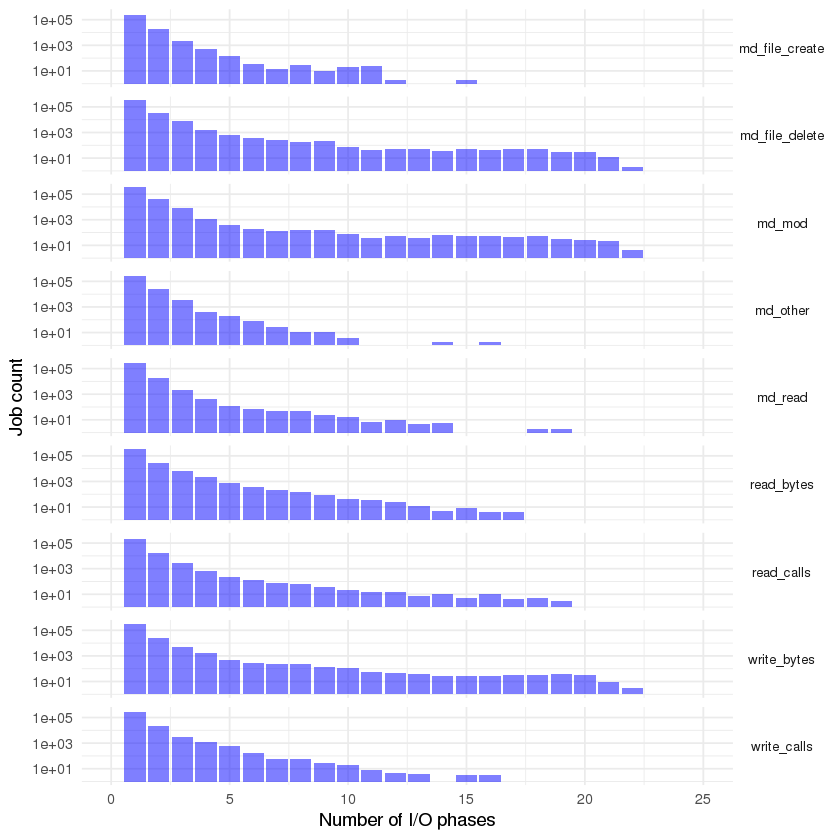
\includegraphics[width=3.55in,height=3.56in]{./media/image23.png}
  \caption{I/O phases statistics.}
  \label{fig:phases_stats}
\end{figure}


\subsection{Evaluation of ML}
This section contains data statistics, and the clustering results in \Cref{fig:datasets_clustering_results} for applying the ML algorithm (hierarchical clustering + decision tree) but using the two different job profiles (IO-Metric and IO-Duration).
Due to lack of tools, we determine cluster quality on a small scale.

\subsubsection{Implementation}
The data is analyzed using Python3.8.0.
In particular we use the agglomerative clustering algorithm, decision trees, and the MinMaxScaler from the scikit-learn 0.22.1 library.


\subsubsection{Results}
We conducted several experiments with different SIM values between 0 and $SIM_{max}$.
The top 20 largest clusters and total number of clusters is visualized in \Cref{fig:datasets_clustering_results:io_metric} and \Cref{fig:datasets_clustering_results:io_duration} for IO-metric and IO-duration job-profiles, respectively.

\begin{figure}
 \begin{subfigure}[t]{0.45\textwidth}
	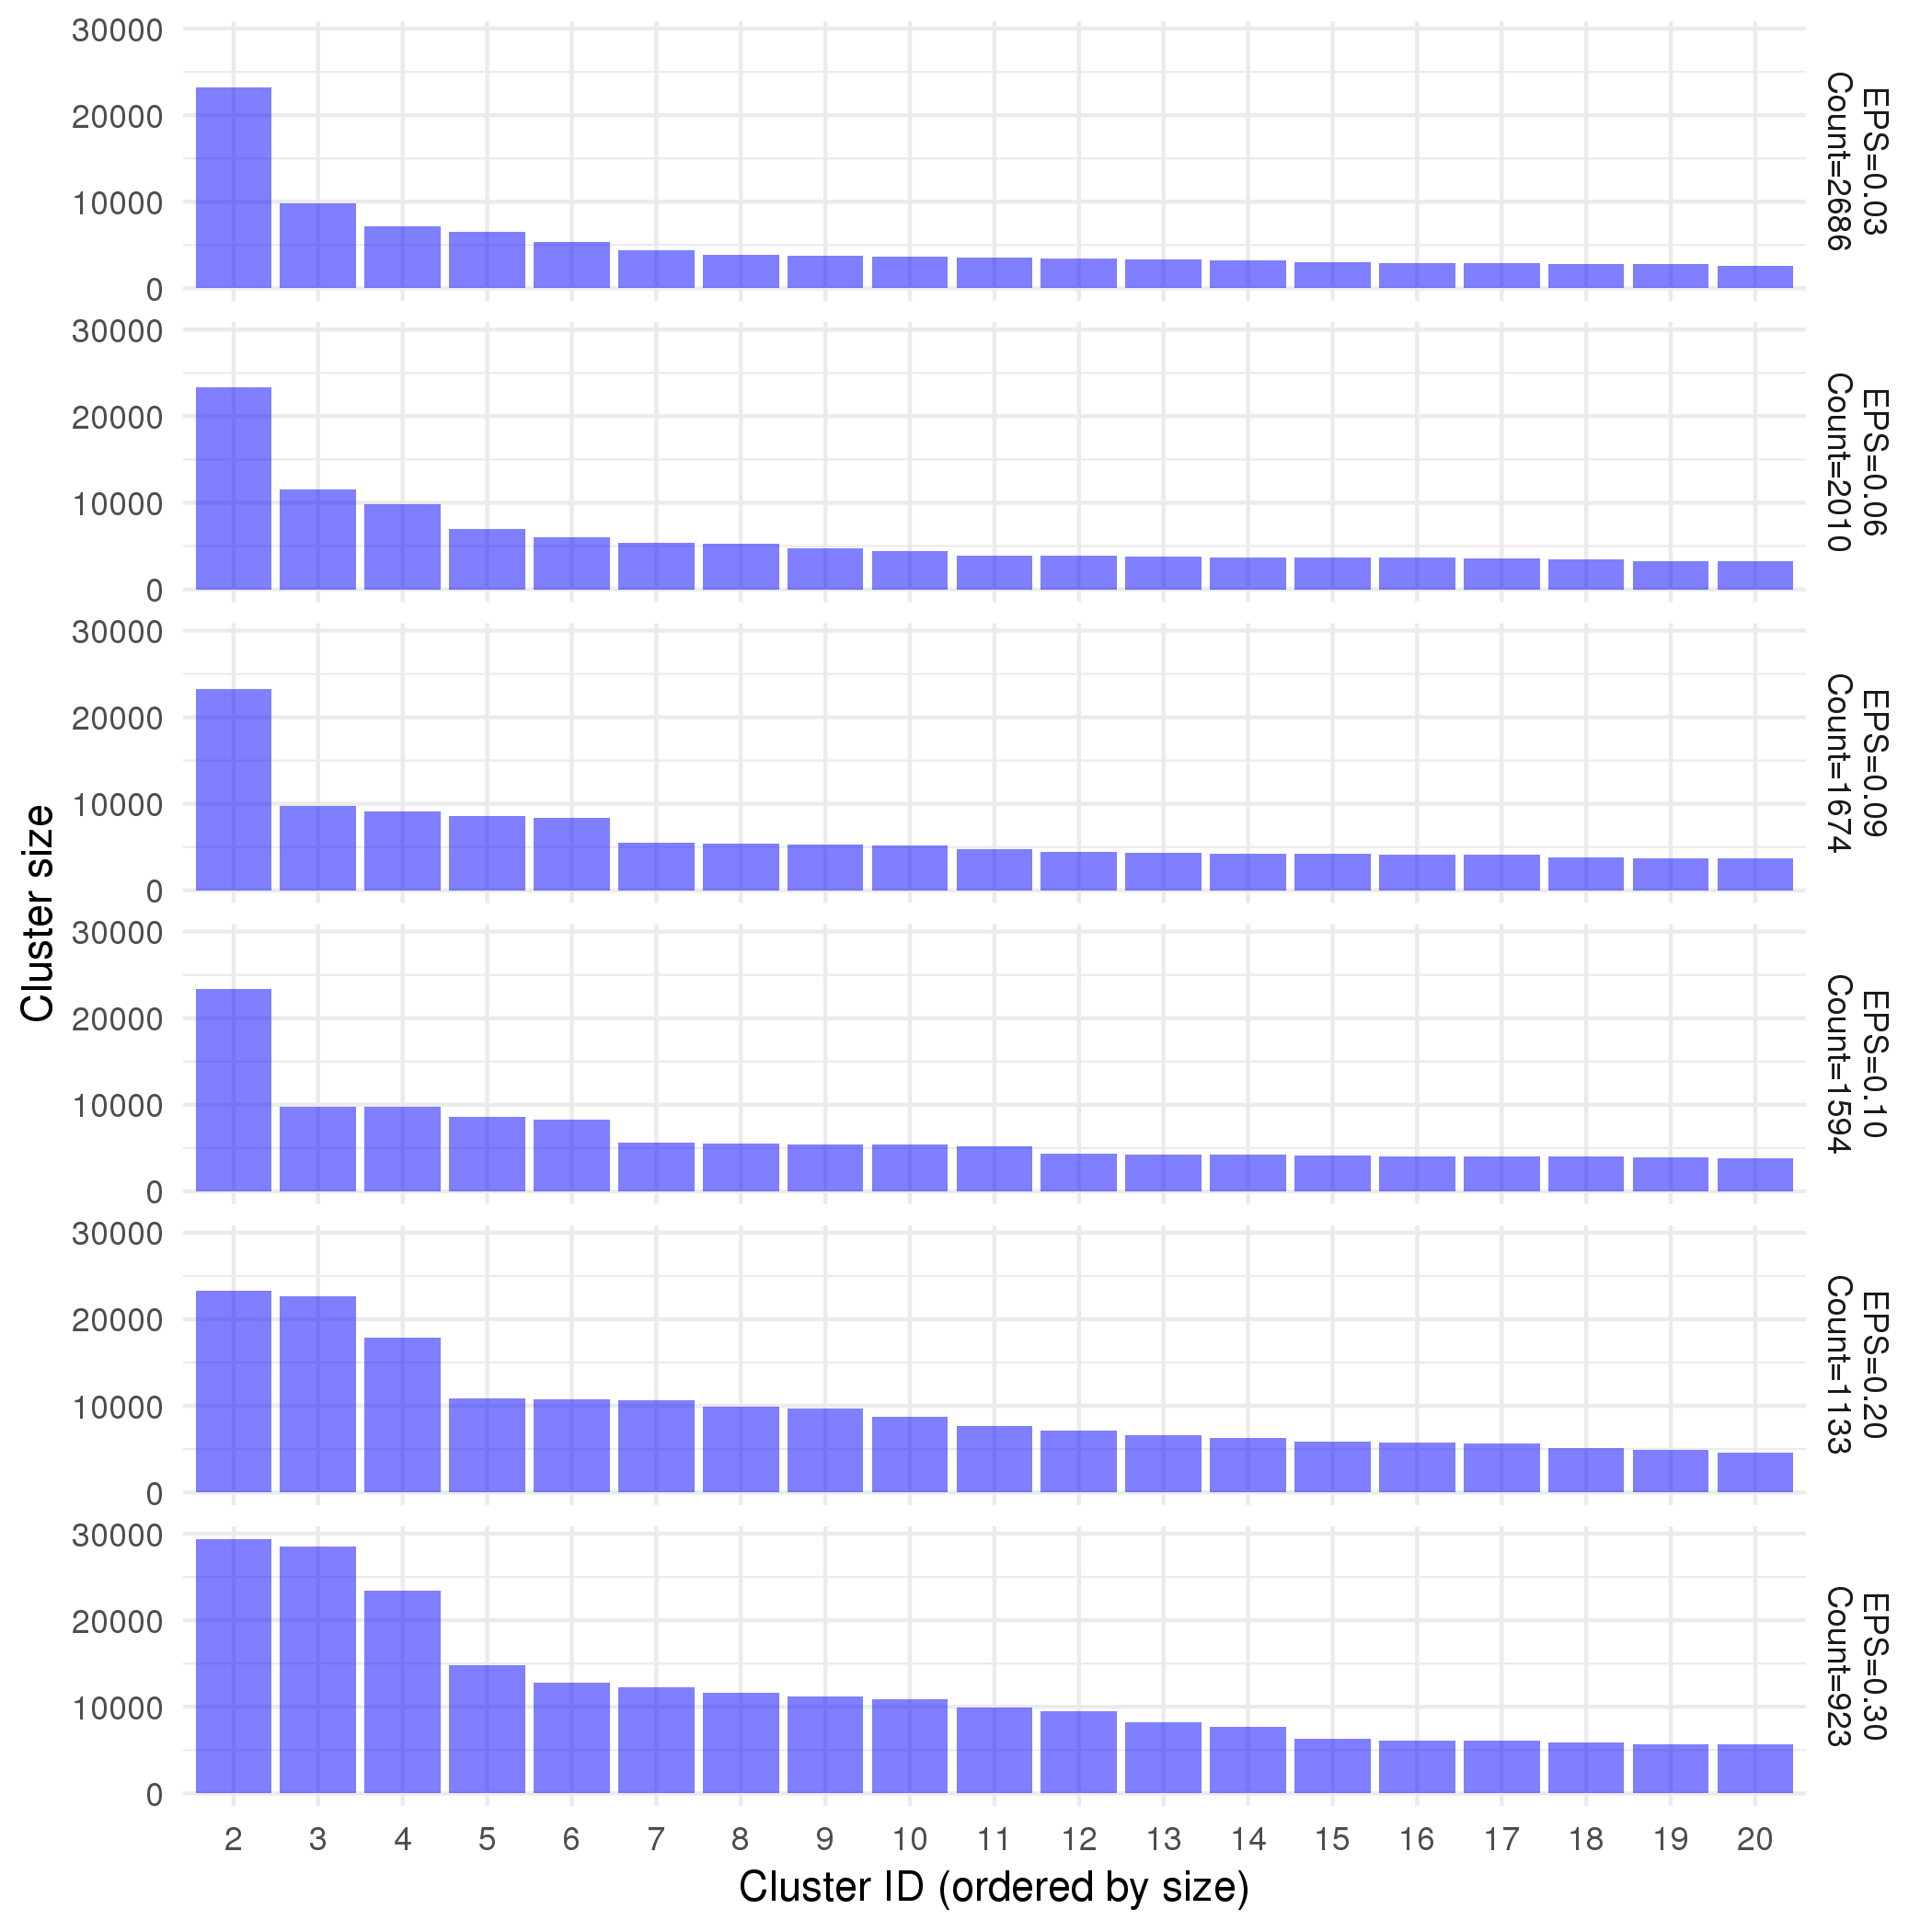
\includegraphics[width=\textwidth]{./media/image12.png}
	\caption{IO-metric}
	\label{fig:datasets_clustering_results:io_metric}
 \end{subfigure}
 \hfill
	\begin{subfigure}[t]{0.45\textwidth}
	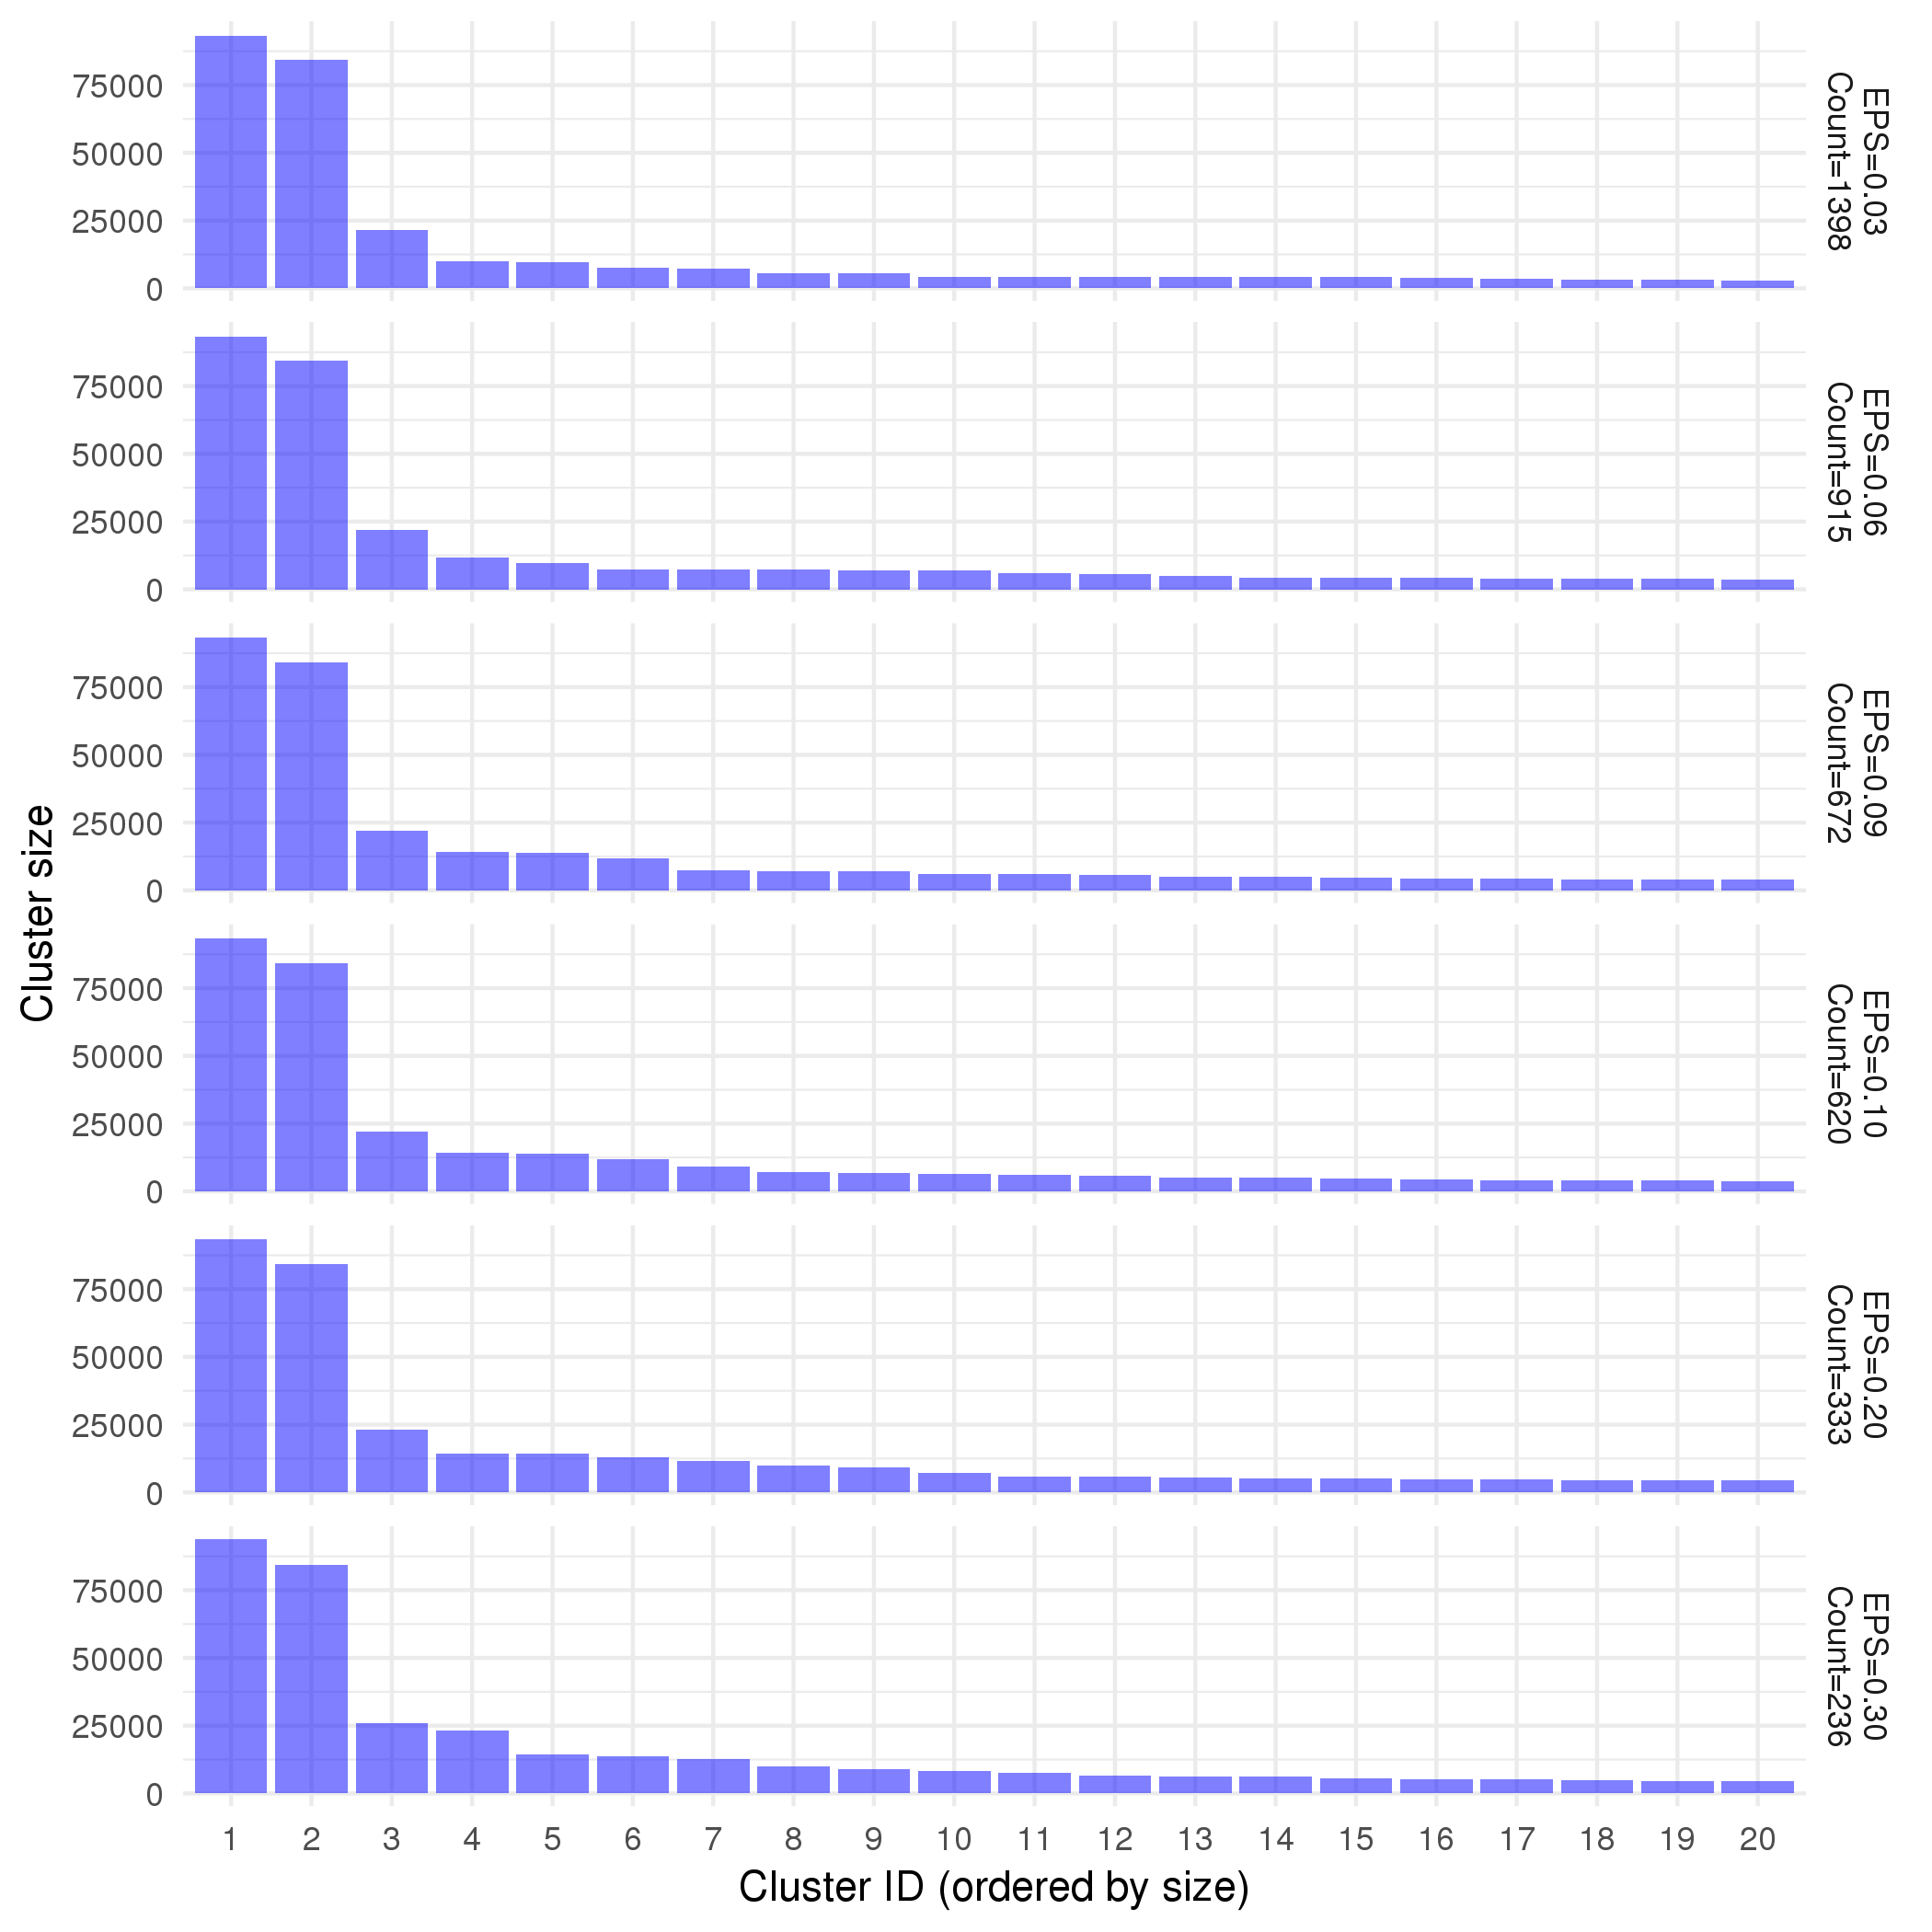
\includegraphics[width=\textwidth]{./media/image10.png}
	\caption{IO-duration}
	\label{fig:datasets_clustering_results:io_duration}
 \end{subfigure}

 \caption{The Top 20 largest clusters for two different job-profiles.}
 \label{fig:datasets_clustering_results}
\end{figure}

\jk{Können wir EPS im Bild durch SIM ersetzen, dann ist das einheitlich.}

We can see that IO-duration generated two very large clusters regardless of SIM.
From Cluster\,3 of IO-duration, the number of jobs inside looks then similar as for IO-metric.
In IO-metric, we can see that with increasing SIM, the number of jobs per cluster increase (as expected).

\jk{Kann es sein, dass EPS=0.3 bei beiden eben nicht das gleiche Verhältnis ist, ich meine SIMmax ist ja unterschiedlich wenn ich 3 Metriken oder 18 habe?}

A look inside clusters reveals chaotic clustering results.
For both datasets and for all SIM values we could find many coding sequences in a cluster that we wouldn't locate together.
For example, one observed cluster contains the following sequences (binary encoding):
\begin{lstlisting}
[1], [0:0:14:0], [4:0], [0:0:4:0], [272:272:272]
\end{lstlisting}

We looked in the Top 10 largest clusters and a random selection of clusters to find the same picture:
Even with low $SIM_{max}$ values the algorithms appears to produce polluted clusters, i.e, with samples from other clusters.
\jk{Warum sim max hier}
Like in the example above, we couldn't understand the logic behind the results.
Probably, the particular random datasets used for training does not represent the specifics of parallel jobs  well enough for proper clustering.
However, even with a good feature set that works on our test system, it is unlikely that the strategy and trained model will be portable to other systems.
Therefore, we conclude that this adapted version of hierarchical clustering based on job profiles isn't suitable to analyze the workload.

\subsection{Evaluation of non-standard clustering algorithms}
This section contains data statistics, clustering progress, and clustering results when applying the five customized algorithms (BIN\_ALL, BIN\_AGGZEROS, HEX\_LEV, HEX\_NATIVE, PM\_QUANT).
%Due to lack of tools, we determine cluster quality on a small scale.

\subsubsection{Test setup}
For the performance tests we allocate a compute node on Mistral supercomputer.
It is equipped with 2x Intel(R) Xeon(R) CPU E5-2680 v3 @ 2.50GHz, 64GB DDR4 RAM.
The clustering algorithms are implemented in Rust and run on a single core.
They are applied on pre-computed codings datasets, so that the clustering runtimes do not include the creation of the codings.

\subsubsection{Quantitative impact of the user-defined similarity}
In the introduced algorithms, the user-defined similarity (SIM) that the jobs in a cluster must fullfill to the cluster centroid controls the cluster formation.
It is expected that low SIM values produce a smaller amount of noisy clusters and a high SIM value produces a large amount of clean clusters.
We suppose the optimal value is application dependent.
Although an optimal SIM value is depending on use case and dataset, a parameter exploration may provide important hints to find a good value and achieve optimal cluster qualities.

\Cref{fig:clustering_progress} shows the number of clusters created when clustering an increasing total number of jobs for different SIM values; each point represents the number for an analyzed number of jobs in increments of 10,000 jobs.
For all algorithms, we can see that with an increase in SIM value, the number of clusters created increases, and the number of total clusters created slows down the more jobs have been processed as jobs are allocated to existing clusters.
BIN creates most clusters while HEX\_NATIVE creates the least and PM is in between.
For SIM of 99\%, BIN and HEX\_LEV can barely group jobs together.


\Cref{fig:alg_runtimes} shows the clustering runtimes for the same experiment.
The clustering time depends heavily on the number of created clusters.
The reason is that the algorithm tries to put each job in existing clusters first.
It iterates over them, and only if it is not able to find a suitable cluster, it creates a new one.
The more clusters exist, the longer is the processing time.
Since, for low SIM values there is a low number of clusters, the clustering is much faster.
PM\_QUANT has exceptionally high runtimes due to quadratic runtimes of phase matching.
In one case, the runtimes clustering of 10,000 jobs took up to 4.3 hours (the few outliers are not shown in the picture).
We suppose this lies on the quadratic runtimes of the phase matching procedure.
% We didn't spend time to optimize the algorithm further.

From this initial considerations, it appears that HEX\_NATIVE is well suited, it generates the least number of clusters and is efficient.
However, looking at the overall number of created clusters isn't enough to assess the quantity of the aggregation.
Additional quantitative metrics need to be used, such as the number of small clusters.

\medskip

To understand the aggregation behavior better, alternative visualizations are investigated.
In \Cref{fig:sim_exploration}, the number of clusters created for a given similarity value is plotted.
The red line approximates the overall number of clusters, the green line shows how many contain at least two jobs and the blue line shows how many of them contain at least 10 jobs.
The maximum number of clusters is equivalent to the number of jobs; it is visualized by the gray line.
Coding with 100$\%$  similarity are of the same job type, i.e, they have exactly the same length and I/O behavior.

The gradient of the curve shows the generalization capabilities of each algorithm for different SIM values.
Apparently, for all algorithms (except HEX) there is a SIM value, where the number of clusters with more than ten and two jobs is decreasing, i.e., the clustering algorithms start to split clusters into individual job clusters.
That is something we usually want to prevent, because the algorithms stop finding similar jobs, but focus on refining clusters.

\smallskip

In \Cref{fig:cum_num_job_sizes}, the distribution of the relative cluster size for all jobs.
The ABS algorithms tend to create many small clusters.
PM creates a variety of different cluster sizes and HEX\_NATIVE the biggest clusters.
Interestingly after scaling both axes with log10, we can observe a linear behavior for all algorithms.

When looking for an optimal SIM, we consider the following criteria:
Firstly, we need to select a SIM value, just before the increase of the SIM value doesn't make significant improvements.
PM and BIN algorithms work best for SIM values between 0.7 and 0.9, and for HEX the SIM value between 0.95 and 0.99.
We can also observe flattening curves with increasing numbers of jobs, which indicates that more jobs are placed in clusters and less clusters are created.
One strategy for the analysis could also be to start with a low SIM value and then increase it further to "hierarchically" cluster jobs and filter jobs that appear irrelevant for the current analysis.

\begin{figure}
  \centering
   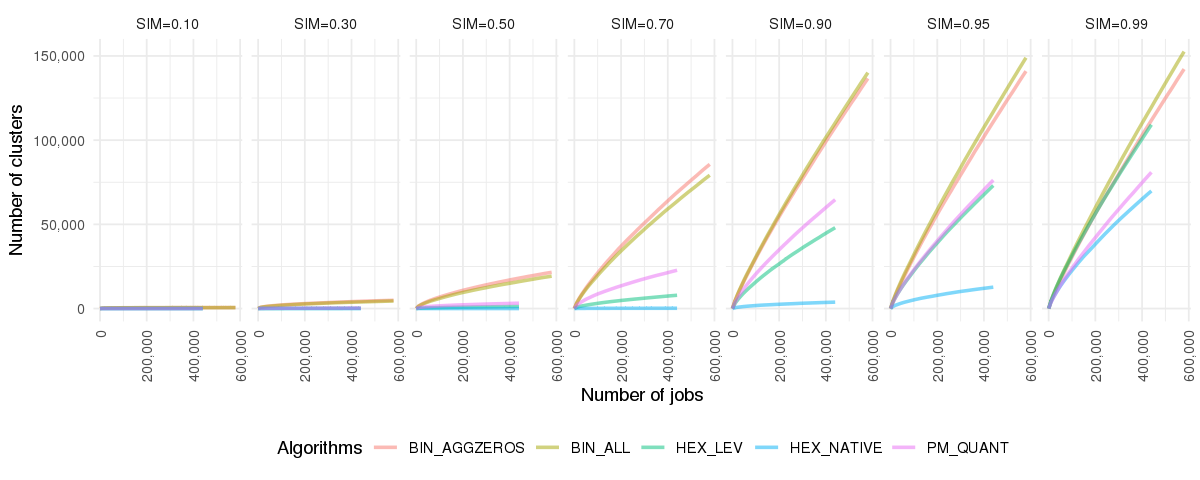
\includegraphics[width=4.61in,height=1.85in]{./media/image15.png}
   \caption{Clustering progress.}
   \label{fig:clustering_progress}
\end{figure}

\begin{figure}
  \centering
  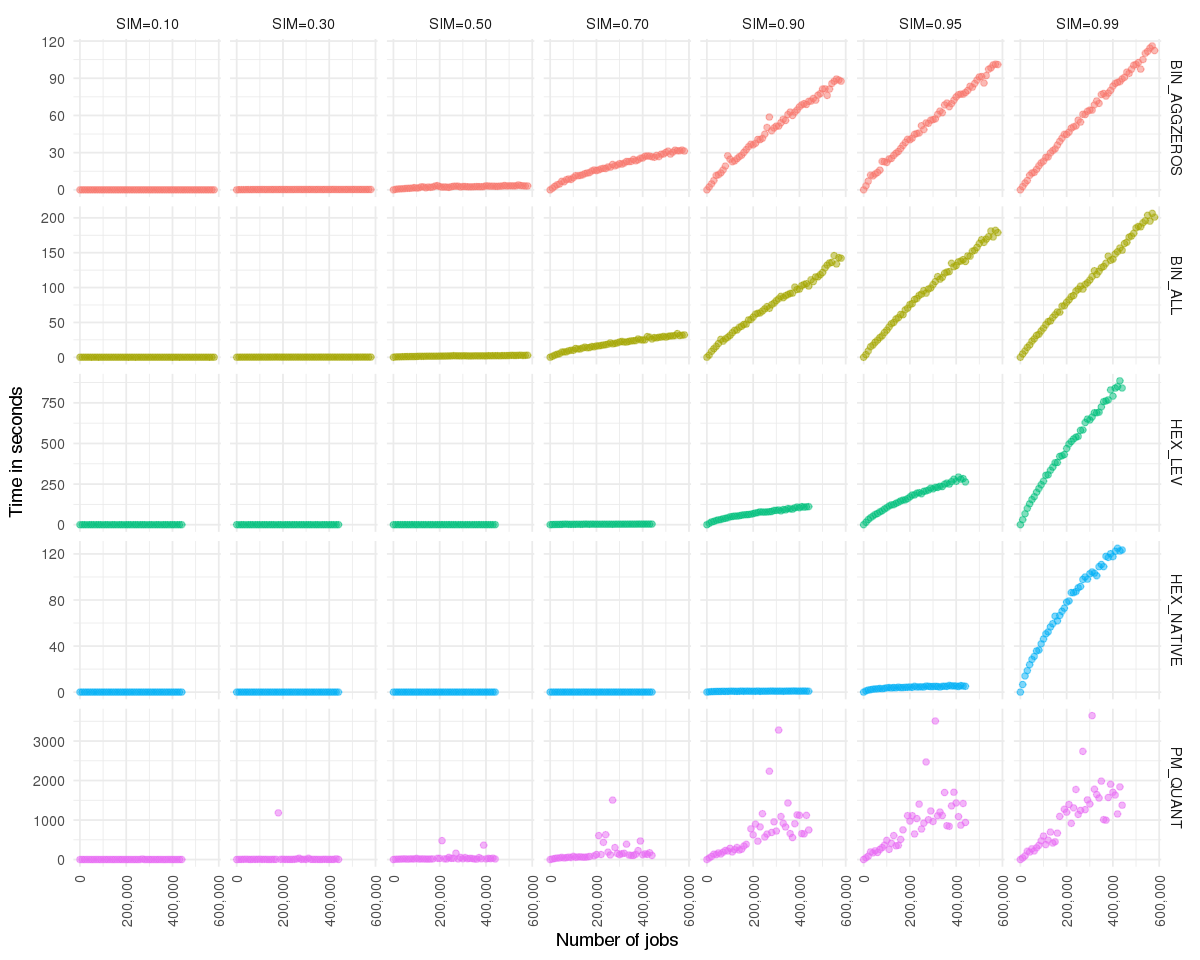
\includegraphics[width=4.61in,height=3.68in]{./media/image18.png}
  \caption{Runtime for executing the clustering.}
  \label{fig:alg_runtimes}
\end{figure}


\begin{figure}
  \centering
  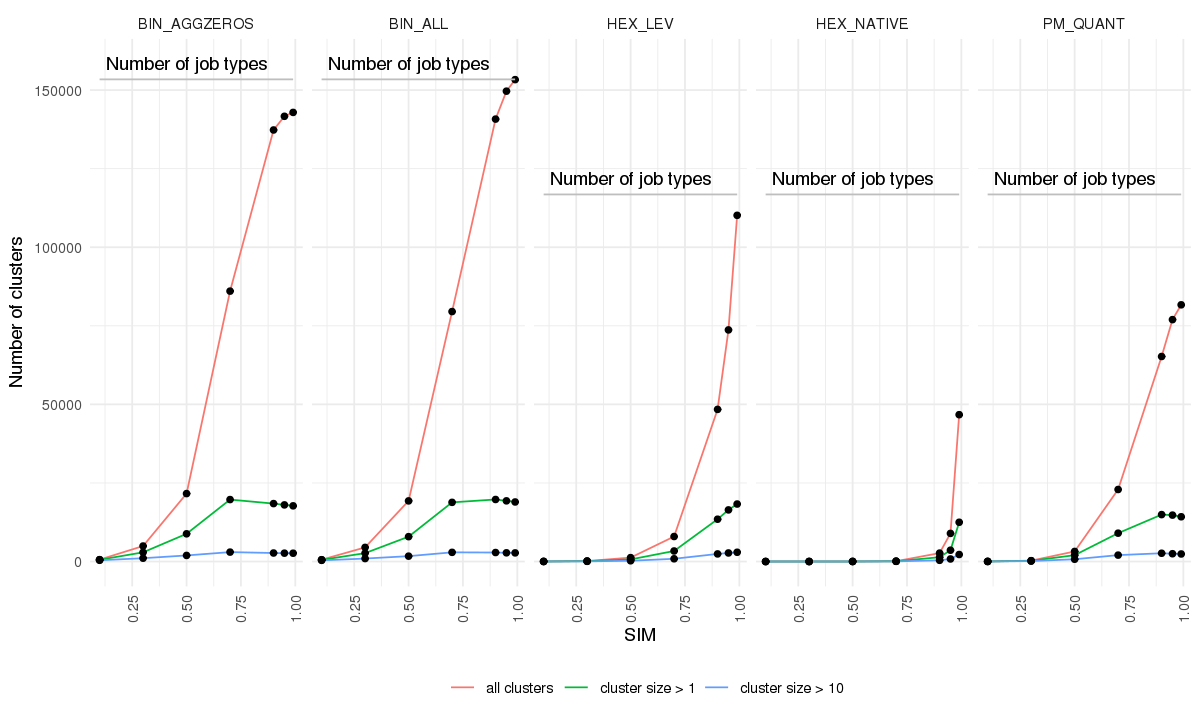
\includegraphics[width=4.61in,height=2.76in]{./media/image19.png}
  \caption{Similarity value exploration.}
  \label{fig:sim_exploration}
\end{figure}

\begin{figure}
  \centering
  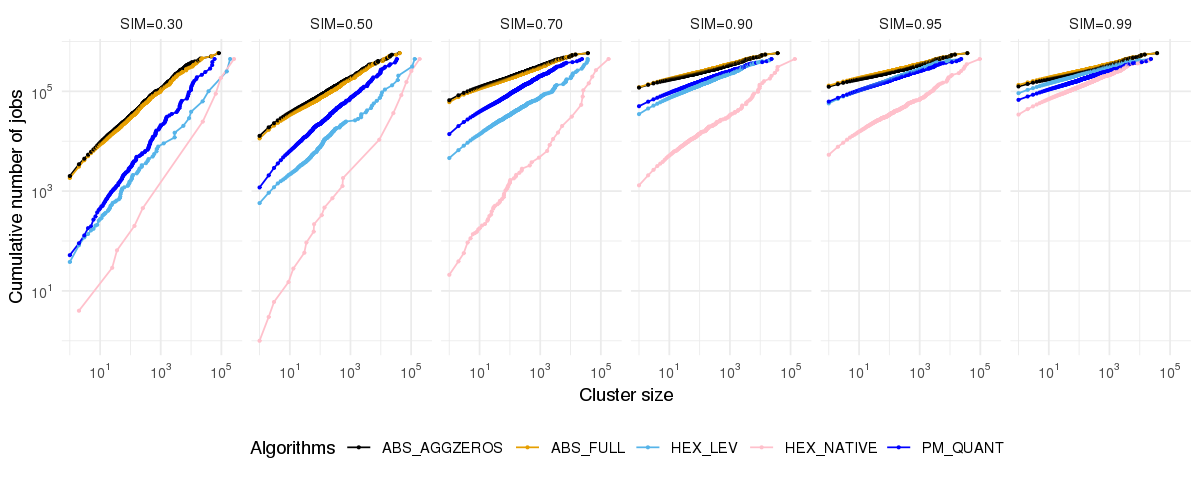
\includegraphics[width=4.61in,height=1.85in]{./media/image22.png}
  \caption{Cumulative number of jobs with different sizes.}
  \label{fig:cum_num_job_sizes}
\end{figure}

\subsection{Cluster relevance}

To assess the quality of the quantitative clustering better and to aid support staff to identify relevant clusters, we define a relevance of clusters as listed in \Cref{eq:rel}.
The idea behind the relevance definition is the following: the larger the cluster (in terms of jobs) and the longer the jobs, the more potential load these jobs can produce.
Therefore, it is worth investigating these clusters first.
Note that the relevance could include the number of occupied nodes as well to effectively indicate the usage of all jobs on the supercomputer.
In this analysis, we just looked at our definition of weighted relevance.

\begin{equation}
\text{Relevance} = \text{ClusterSize} \cdot \text{MeanJobLenght}
\label{eq:rel}
\end{equation}

To give you an impression of cluster qualities for different SIM values, we visualize the Top 10 relevant clusters in \Cref{fig:top10_relevant_jobs}.
The colors indicate the mean similarity of jobs to the cluster centroid.
The number above the bar denotes the mean job length of the cluster.

In principle, the figure confirms that SIM values larger than optimum provide not much improvement, but nevertheless, it does not mean that the cluster quality is acceptable.
After manual exploration of selected clusters, we noticed some show a SIM-value independent characteristics.
To explain them, it is sufficient to investigate one cluster in detail for each algorithm, as we do in the next sections.

%\begin{figure}
%  \centering
%  
\includegraphics[width=2.5in,height=0.12in]{./media/image16.png}
%  \caption{Equation}
%  \label{fig:equation}
%\end{figure}

\begin{figure}
  \centering
   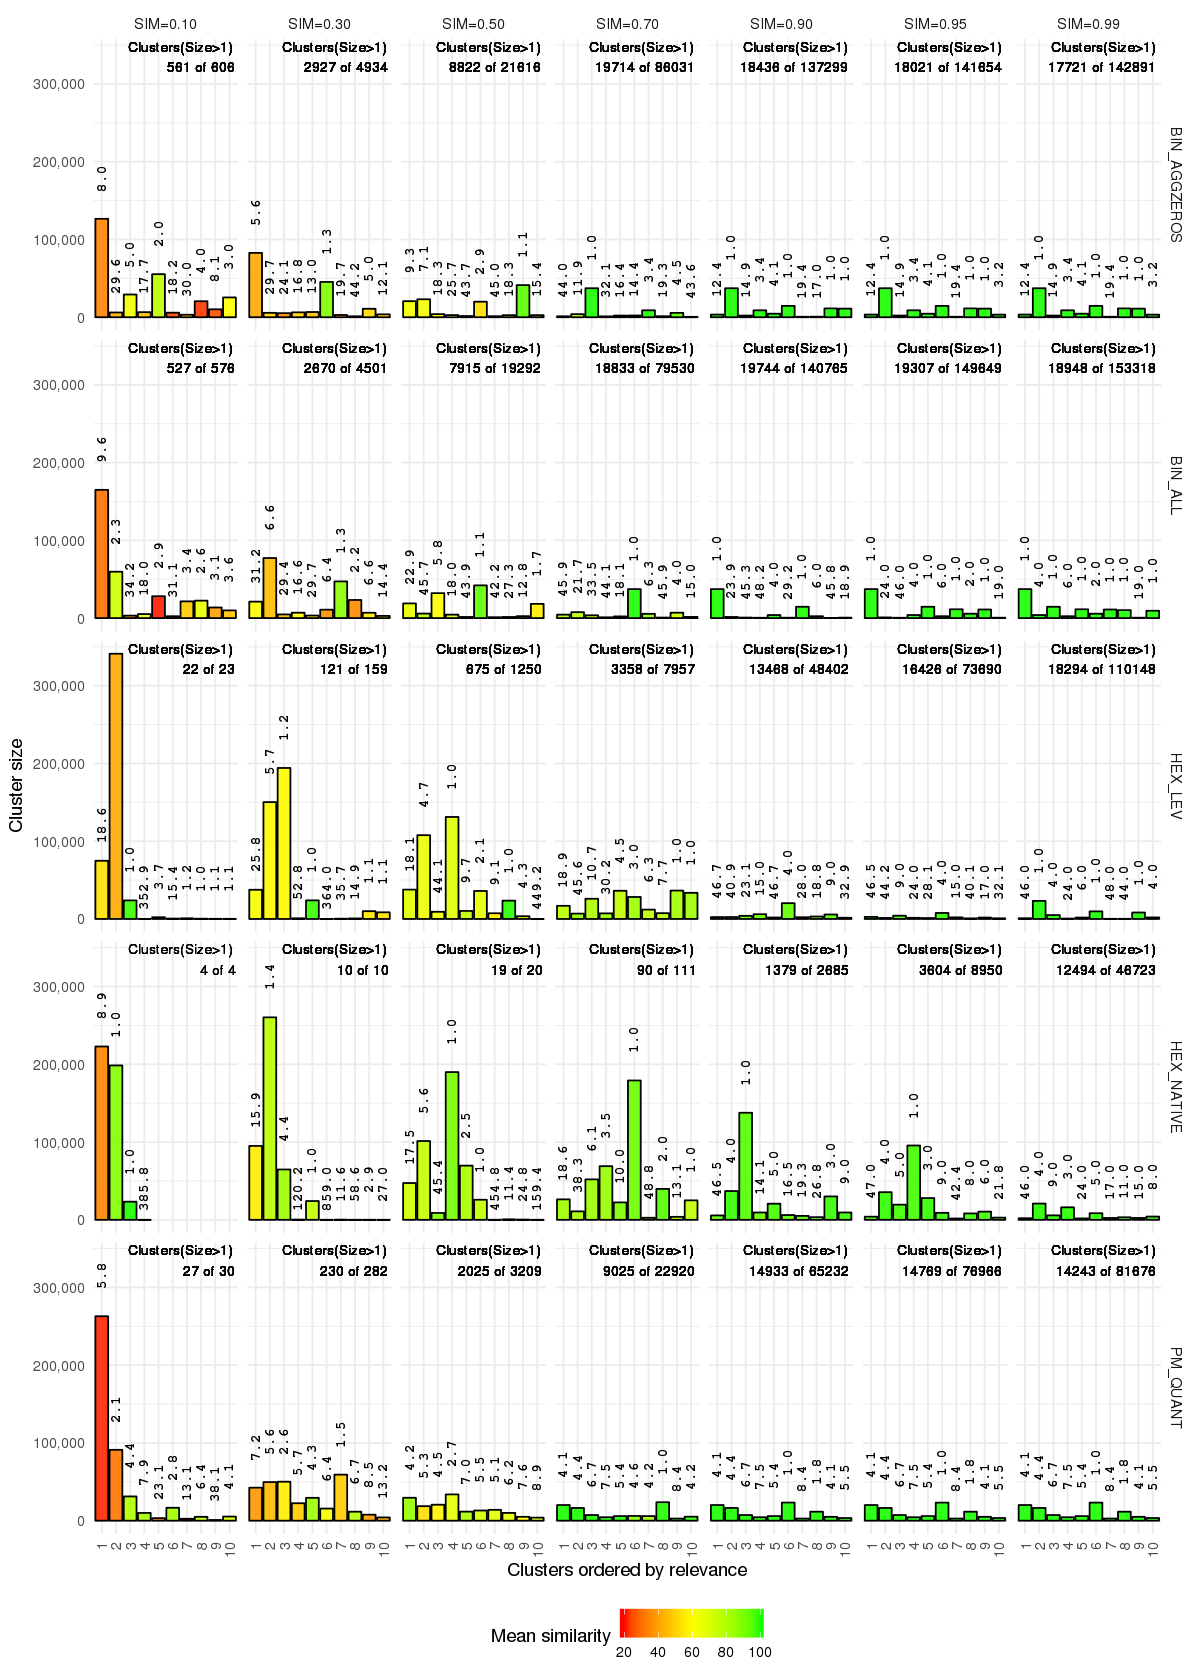
\includegraphics[width=4.61in,height=6.44in]{./media/image11.png}
   \caption{Top 10 relevant jobs ordered by relevance.}
   \label{fig:top10_relevant_jobs}
\end{figure}

\jk{END of review}

\subsubsection{Cluster presentation format}
The next sections we have the following format, a description of any particular observations if necessary, followed by a table containing the most important statistics, and by the codings for job, centroid and and the Top 5 job types.
At the end we include an illustration which describes the length distribution of the cluster.
\subsubsection{Algorithm characteristics}
\paragraph{BIN\_ALL}
Information related to the cluster is in \Cref{tab:bin:largest_clusters}, \Cref{tab:bin_all:stats}, \Cref{tab:bin_all:top_jobs}, and \Cref{fig:bin_all:length}.
One of the first observations we did for BIN family algorithms is that the six largest clusters contain the shortest jobs (one segment long).
They are listed in \Cref{tab:bin:largest_clusters}.
All jobs in each cluster have exactly the same codings.
The reason that both algorithms create the same clusters, is that the zero aggregation has no effect on formation of these clusters, because the jobs are too short (the minimum job length required for effective zero aggregation is at least three segments) and that the dataset contains a vast amount of such jobs.
The largest cluster is even representative in Top10 relevant jobs in ref\_top\_ten.

%\begin{table}[h]
\begingroup
  \centering
  \begin{tabular}{ll}
    Coding sequence & Cluster size \\
    \hline
    $[511]$ & 37,272 \\
    $[32]$  & 14,536 \\
    $[272]$ & 11,338 \\
    $[160]$ & 11,014 \\
    $[128]$ & 10,228 \\
    $[8]$   & 9,446  \\
  \end{tabular}
  \captionof{table}{Top 6 largest clusters created by BIN algorithms with SIM = 0.7.}
  \label{tab:bin:largest_clusters}
\endgroup
%\end{table}

Most jobs in the cluster are shorter than 49 segments, because the main Mistral partitions can allocate jobs for at most 8 hours, and that is the majority of jobs.
The other jobs must be special allocations.
Since each segment is 10 min long, the runtime of jobs with 49 segments is about 8.16 hours.
The other jobs must be special allocations or jobs from other partitions.

The following observations are characteristic for this algorithm:
\begin{enumerate}
 \item Job types can significantly differ from centroid and from each other.
 \item Lengths of job types in a cluster are relatively close to the centroid.
\end{enumerate}

%\begin{table}[h]
\begingroup
  \centering
  \begin{tabular}{lr}
    SIM & 0.7 \\
    Number of jobs & 7615 \\
    Number of job types & 3306 \\
  \end{tabular}
  \captionof{table}{Cluster statistics.}
  \label{tab:bin_all:stats}
\endgroup
%\end{table}

%\begin{table}[h]
\begingroup
  \centering
  \begin{tiny}
    \begin{tabular}{@{ }l@{ }|@{ }r@{ }}
      \rowcolor{tabhcolor}
      Binary coding                                                                                    &  Type     \\
      \hline
      0:0:0:0:0:0:294:0:0:0:0:32:0:0:0:0:0:0:0:0:0:0:0:32:0:0:0:0:0:0:0:0:0:0:0:32:0:0:0:0:0:0:0:0:0:0 &  centroid \\
      \multicolumn{2}{l}{}                                                                             \\
      \rowcolor{tabhcolor}
      Binary coding                                                                                    &  Count    \\
      \hline
      0:0:0:0:0:0:359:96:0:0:0:0:0:0:0:0:0:0:0:0:0:0:0:0:0:0:0:0:0:0:0:0:0:0:0:0:0:0:0:0:0:0:0:0:0:0   &  95       \\
      0:0:0:0:0:0:295:0:0:0:0:0:0:0:0:0:0:0:0:0:0:0:0:0:0:0:0:0:0:0:0:0:0:0:0:0:0:0:0:0:0:0:0:0:0:0    &  62       \\
      0:0:0:0:0:0:0:0:0:0:0:0:4:0:0:0:0:0:0:0:0:0:0:0:0:0:0:0:0:0:0:0:0:0:0:0:0:0:0:0:0:0:0:0:0:0:0:0  &  47       \\
      0:0:0:0:0:0:359:0:0:0:0:0:0:0:0:0:0:0:0:0:0:0:0:0:0:0:0:0:0:0:0:0:0:0:0:0:0:0:0:0:0:0:0:0:0:0    &  44       \\
      0:0:0:0:0:6:6:0:0:0:0:0:0:0:0:0:0:0:0:0:0:0:0:0:0:0:0:0:0:0:0:0:0:0:0:0:0:0:0:0:0:0:0:0:0:0:0:0  &  40       \\
    \end{tabular}
  \end{tiny}
  \captionof{table}{Centroid and Top 5 job types.}
  \label{tab:bin_all:top_jobs}
\endgroup
%\end{table}

%\begin{figure}[h]
\begingroup
  \centering
  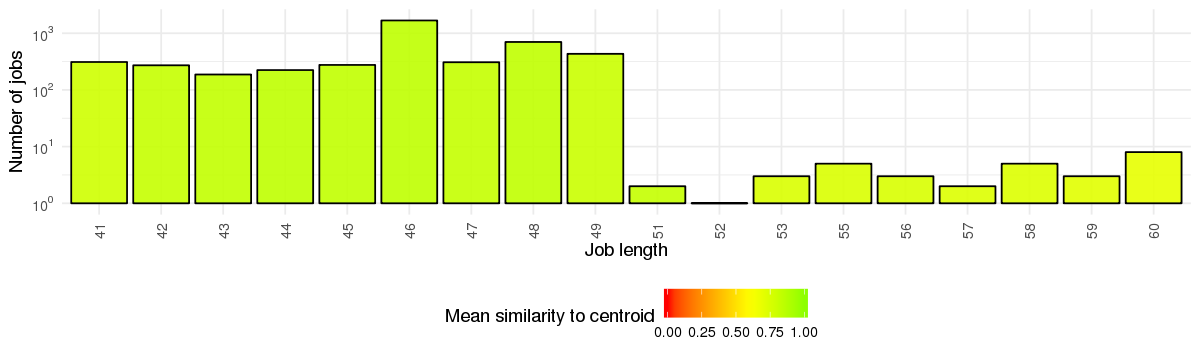
\includegraphics[width=4.61in,height=1.39in]{./media/image20.png}
  \captionof{figure}{Length distribution in the cluster.}
  \label{fig:bin_all:length}
\endgroup
%\end{figure}

\paragraph{BIN\_AGGZEROS}
Information related to the cluster is in \Cref{tab:bin_aggzeros:stats}, \Cref{tab:bin_aggzeros:top_jobs}, and in \Cref{fig:bin_aggzeros:length}.
The following is characteristic for this algorithm:

\begin{enumerate}
 \item Job types can significantly differ from centroid and from each other.
 \item Lengths of job types in a cluster are relatively far from the centroid and compared to BIN\_ALL.
 \item I/O intensive clusters appear to be cleaner than BIN\_ALL.
\end{enumerate}


%\begin{table}[h]
\begingroup
  \begin{tabular}{ll}
    \centering
    SIM &  0.7 \\
    Number of jobs & 1295 \\
    Number of job types & 336 \\
  \end{tabular}
  \captionof{table}{Cluster statistics.}
  \label{tab:bin_aggzeros:stats}
\endgroup
%\end{table}

%\begin{table}[h]
\begingroup
  \centering
  \begin{tiny}
    \begin{tabular}{@{ }l@{ }|@{ }r@{ }}
      \rowcolor{tabhcolor}
      Binary coding                                                                          &  Type     \\
      \hline
      272:272:272:272:272:278:286:272:272:272:272:272:272:272:272:272:272:272:272            &  centroid \\
      \multicolumn{2}{l}{}                                                                   \\
      \hline
      \rowcolor{tabhcolor}
      Binary coding                                                                          &  Count    \\
      272:272:272:272:272:278:286:272:272:272:272:272:272:272:272:272:272:272:272            &  528      \\
      272:272:272:272:272:406:286:272:272:272:272:272:272:272:272:272                        &  96       \\
      272:272:272:272:272:279:31:272:272:272:272:272:272:272:272:272:272:272:272:272:272:272 &  53       \\
      272:272:272:272:272:272:272:272:272:272:272:279:319:272:272:272:272:272:272:272:272    &  52       \\
      272:272:272:272:272:279:319:272:272:272:272:272:272:272:272:272:272:272:272:272:272    &  50       \\
    \end{tabular}
  \end{tiny}
  \captionof{table}{Centroid and Top 5 job types}
  \label{tab:bin_aggzeros:top_jobs}
\endgroup
%\end{table}

%\begin{figure}[h]
\begingroup
  \centering
  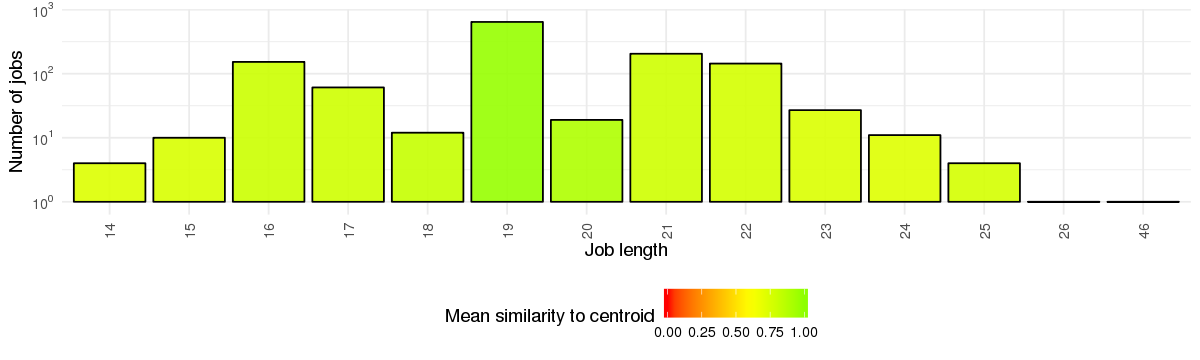
\includegraphics[width=4.61in,height=1.38in]{./media/image13.png}
  \captionof{figure}{Job length distribution in the cluster.}
  \label{fig:bin_aggzeros:length}
\endgroup
%\end{figure}

\paragraph{HEX\_LEV}
Information related to the cluster is in \Cref{tab:hex_lev:stats}, \Cref{tab:hex_lev:top_jobs}, and in \Cref{fig:hex_lev:length}.
HEX\_LEV reacts slowly to the increasing SIM value, due to the longer hexadecimal codings, compared to binary codings.
Therefore, we chose a SIM value higher than for BIN algorithms.
But even with a high SIM value, we can observe that some jobs have a different I/O behavior than the centroid and the rest of the jobs.
The reason is that Levenshtein distance is not performance aware, i.e., the distance between value 1 and 2 is the same as for 1 and 8.
There is no such a job in the example below, but we can observe this in other clusters.
Cluster characteristics:

\begin{enumerate}
 \item Similar job lengths
 \item Mostly clean clusters, but can contain outlier jobs
\end{enumerate}
%\begin{table}[h]
\begingroup
	\centering
	\begin{tabular}{ll}
		SIM & 0.9 \\
		Number of jobs & 5769 \\
		Number of job types & 2473 \\
	\end{tabular}
	\captionof{table}{Cluster statistics.}
	\label{tab:hex_lev:stats}
\endgroup
%\end{table}

%\begin{table}[h]
\begingroup
  \centering
  \begin{tiny}
    \begin{tabular}{@{ }l@{ }@{ }l@{ }@{ }l@{ }@{ }l@{ }|@{ }r@{ }}
      \rowcolor{tabhcolor}
      \multicolumn{4}{@{ }l|@{ }}{Hexadecimal coding} & \\
      \rowcolor{tabhcolor}
      md\_file\_create  & md\_file\_delete  & md\_mod           & read\_calls       & Type     \\
      \hline
      0:...:0           & 0:0:0:1:0:0:0:0:0 & 0:...:0           & 0:...:0           & centroid \\
      \multicolumn{5}{l}{}\\
      \rowcolor{tabhcolor}
      md\_file\_create  & md\_file\_delete  & md\_mod           & read\_calls       & Count    \\
      \hline
      0:...:0           & 0:0:0:0:0:0:1:0:0 & 0:...:0           & 0:...:0           & 606      \\
      0:...:0           & 0:0:0:0:0:0:0:0:1 & 0:...:0           & 0:...:0           & 562      \\
      0:...:0           & 0:...:0           & 0:...:0           & 0:0:0:0:0:0:1:0:0 & 429      \\
      0:...:0           & 0:0:0:1:0:0:0:0:0 & 0:...:0           & 0:...:0           & 185      \\
      0:0:0:0:0:0:1:1:1 & 0:...:0           & 0:0:0:0:0:0:1:0:0 & 0:...:0           & 75       \\
    \end{tabular}
  \end{tiny}
  \captionof{table}{Centroid and Top 5 job types}
  \label{tab:hex_lev:top_jobs}
\endgroup
%\end{table}

%\begin{figure}[h]
\begingroup
  \centering
  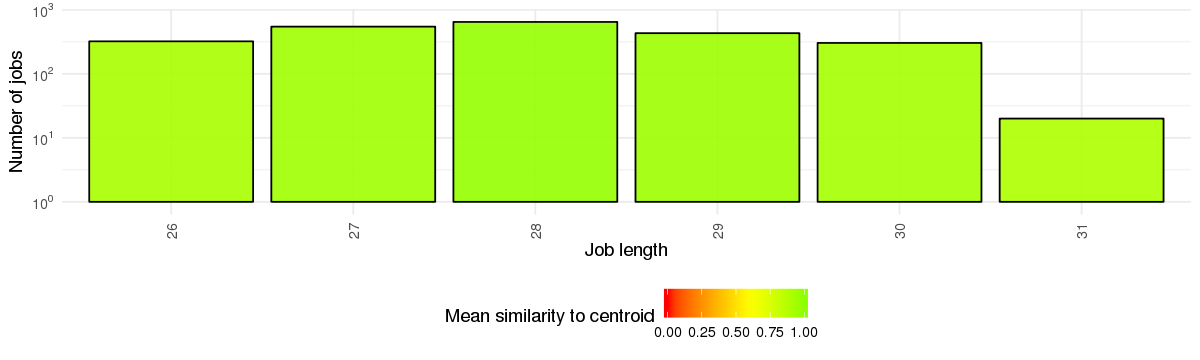
\includegraphics[width=4.61in,height=1.39in]{./media/image5.png}
  \captionof{figure}{Length distribution in the cluster.}
  \label{fig:hex_lev:length}
\endgroup
%\end{figure}

\paragraph{HEX\_NATIVE}
Information related to the cluster is in \Cref{tab:hex_native:stats}, \Cref{tab:hex_native:top_jobs}, and in \Cref{fig:hex_native:length}.
The SIM value exploration shows that this algorithm works best with high SIM values.
Clustering with SIM=0.99 results in clusters that have equal job lengths.
(For SIM=0.99 the centroid must be longer than 100 segments to attract jobs with other lengths.)Cluster characteristics:
\begin{enumerate}
 \item Similar job lengths
 \item Jobs are relatively close to the centroid
 \item Low number of outliers
\end{enumerate}

%\begin{table}[h]
\begingroup
  \centering
  \begin{tabular}{ll}
    SIM & 0.99 \\
    Number of jobs & 20908 \\
    Number of job types & 11997 \\
  \end{tabular}
  \captionof{table}{Cluster statistics.}
  \label{tab:hex_native:stats}
\endgroup
%\end{table}

%\begin{table}[h]
\begingroup
  \centering
  \begin{tiny}
    \begin{tabular}{@{ }l@{ }@{ }l@{ }@{ }l@{ }|@{ }r@{ }}
      \rowcolor{tabhcolor}
      \multicolumn{3}{@{ }l|@{ }}{Hexadecimal coding} &            \\
      \rowcolor{tabhcolor}
      md\_file\_delete     &  md\_mod   & md\_other & Type     \\
      \hline
      0:\dots:0            &  0:0:1:0   & 0:0:1:0   & centroid \\
      \multicolumn{4}{l}{} \\
      \rowcolor{tabhcolor}
      md\_file\_delete     &  md\_mod   & md\_other & Count    \\
      \hline
      0:\dots:0            &  0:\dots:0 & 0:0:1:0   & 5,010    \\
      0:\dots:0            &  0:\dots:0 & 0:0:2:0   & 1,963    \\
      0:0:1:0              &  0:\dots:0 & 0:\dots:0 & 1,099    \\
      0:\dots:0            &  0:\dots:0 & 0:1:0:0   & 911      \\
      0:0:1:0              &  0:0:1:0   & 0:\dots:0 & 676      \\
    \end{tabular}
  \end{tiny}
  \captionof{table}{Centroid and Top 5 job types.}
  \label{tab:hex_native:top_jobs}\endgroup
%\end{table}

%\begin{figure}[h]
\begingroup
  \centering
  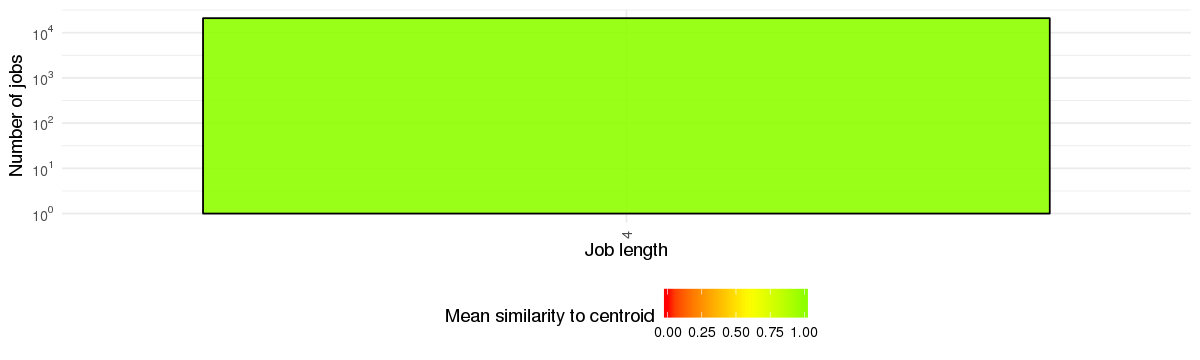
\includegraphics[width=4.61in,height=1.39in]{./media/image8.png}
  \captionof{figure}{Length distribution in the cluster.}
  \label{fig:hex_native:length}
\endgroup
%\end{figure}

\paragraph{PM\_QUANT}
Information\ related to the cluster is in \Cref{fig:pm_quant:stats}, \Cref{fig:pm_quant:top_jobs}, and in \Cref{fig:pm_quant:length}.
The first thing to mention are the high generalization capabilities of the algorithm, i.e., that many jobs are mapped to a relatively low number of types.
The next typical property is shown in \Cref{fig:pm_quant:length}, where we can see that almost the full range of job lengths is represented in the cluster.
This happens, because the PM ignores zero segments completely.
We saw that already in BIN\_AGGZEROS, where a similar effect was caused by the aggregation of zero segments.
For example, for PM, the job types in \Cref{fig:pm_quant:top_jobs} in the row one and two are 100$\%$  similar.
Remarkable is also the cleanliness of the clusters.
The centroid and the jobs contain quite similar I/O patterns.
Cluster characteristics:


\begin{enumerate}
 \item Low number of job types
 \item Relatively large number of job lengths
 \item I/O pattern
\end{enumerate}

%\begin{table}[h]
\begingroup
  \centering
  \begin{tabular}{ll}
    SIM & 0.7 \\
    Number of jobs & 5175 \\
    Number of job types & 154 \\
  \end{tabular}
  \captionof{table}{Cluster statistics.}
  \label{fig:pm_quant:stats}
\endgroup
%\end{table}

%\begin{table}[h]
\begingroup
  \centering
  \begin{tiny}
    \begin{tabular}{@{ }l@{ }@{ }l@{ }|@{ }r@{ }}
      \rowcolor{tabhcolor}
      \multicolumn{2}{@{ }l|@{ }}{Hexadecimal coding} &              \\
      \rowcolor{tabhcolor}
      md\_file\_delete     &  md\_mod     & Type     \\
      \hline
      4:0:0:0:0:0          &  4:0:0:0:0:0 & centroid \\
      \multicolumn{3}{l}{} \\
			\rowcolor{tabhcolor}
      md\_file\_delete     &  md\_mod     & Count    \\
      \hline
      4                    &  4           & 2329     \\
      4:0:0:0:0:0          &  4:0:0:0:0:0 & 1773     \\
      4:0                  &  4:0         & 224      \\
      2                    &  4           & 65       \\
      0:4                  &  0:4         & 57       \\
    \end{tabular}
  \end{tiny}
  \captionof{table}{Centroid and Top 5 job types.}
  \label{fig:pm_quant:top_jobs}
\endgroup
%\end{table}

%\begin{figure}[h]
\begingroup
  \centering
  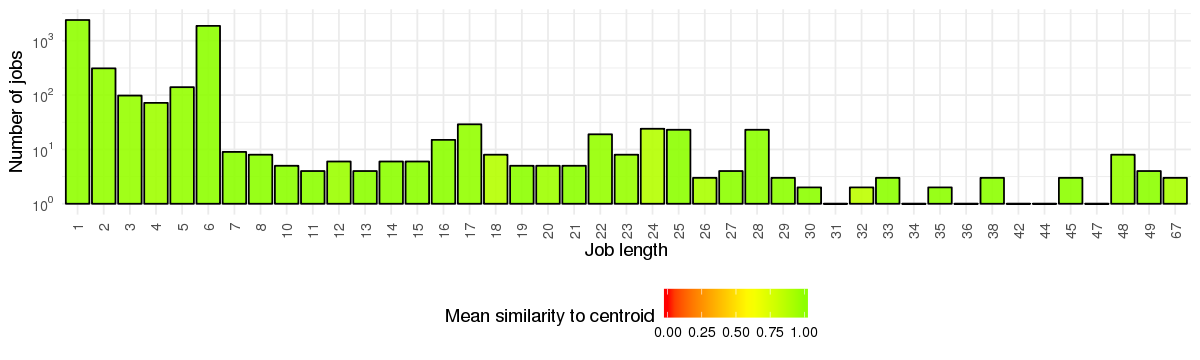
\includegraphics[width=4.61in,height=1.39in]{./media/image21.png}
  \captionof{figure}{Length distribution in the cluster.}
  \label{fig:pm_quant:length}
\endgroup
%\end{figure}

\subsection{Use case: I/O intensive job}
The demonstration in this section shows how this approach can be used to identify a cluster of I/O-intensive jobs similar to an existing job.

\begin{figure}[h]
  \centering
  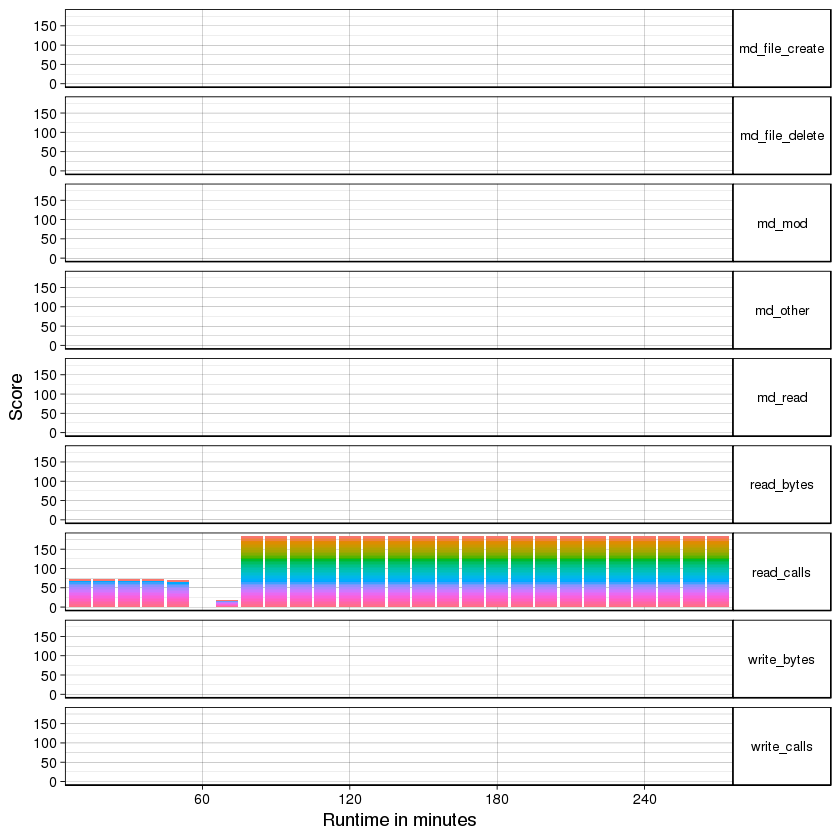
\includegraphics[width=2.84in,height=2.85in]{./media/image1.png}
  \caption{One high I/O intensity job running on 46 nodes. Score is the sum of all nodes stacked by the node. A color represents one of the nodes.}
  \label{fig:use_case}
\end{figure}

Firstly, we find an I/O intensive job that we use to identify similar jobs.
The selected job is visualized in \Cref{fig:use_case}.
We can see that this job reads data over the whole runtime.
At beginning, only a subset of the nodes is reading most of the data, later more nodes participate in the reading The amount of transmitted data is not large, but the amount of read calls is exceptionally high and may potentially degrade the file system performance.
Now we investigate the cluster that contains this job for the different algorithms.

In the following, an attentive reader may notice that there is a discrepancy between the job visualization in  \Cref{fig:use_case} and the hexadecimal job codings.
While in the figure we can see a less intensive phase in the beginning and a high intensive phase afterwards, the hexadecimal coding contains a more or less single high intensive I/O phase.
The reason is that we use different reduction functions. While in the illustration we aggregate segments by the sum() function, for the coding we use mean() function for the same set of values.
While sum() is better for visualization, the mean value allows us to build simple algorithms.

By accident, we have good conditions for all algorithms, and all the algorithms work well in this use case.
We have a relatively long job with one heavily used metric, and we can identify a cluster with similar jobs.
We omit comments.
The reader can make up his own mind.
\paragraph{BIN\_ALL}
Information related to the cluster is in \Cref{tab:use_case:bin_all:stats}, \Cref{tab:use_case:bin_all:top_jobs}, and in \Cref{fig:use_case:bin_all:length}.

%\begin{table}[h]
\begingroup
  \centering
  \begin{tabular}{ll}
    SIM & 0.7 \\
    Number of jobs & 27 \\
    Number of job types & 17 \\
  \end{tabular}
  \captionof{table}{Cluster statistics.}
  \label{tab:use_case:bin_all:stats}
\endgroup
%\end{table}

%\begin{table}[h]
\begingroup
  \centering
  \begin{tiny}
    \begin{tabular}{@{ }l@{ }|@{ }r@{ }}
      \rowcolor{tabhcolor}
      Binary coding                                                                                          &  Type     \\
      \hline
      192:192:192:192:192:192:196:192:192:192:192:192:192:192:192:192:192:192:192:192:192:192:64:64:64:64:64 &  job      \\
      192:192:192:192:192:192:192:192:192:192:192:454:230:192:192:192:192:192:192:192:192:192:192:192        &  centroid \\
      \multicolumn{2}{l}{}                                                                                   \\
      \rowcolor{tabhcolor}
      Binary coding                                                                                          &  Count    \\
      \hline
      192:192:192:192:192:454:198:192:192:192:192:192:192:192:192:192:192:192:192:192:192:192:192:192        &  5        \\
      192:192:192:192:192:192:192:192:192:192:192:454:230:192:192:192:192:192:192:192:192:192:192:192        &  3        \\
      192:192:192:192:192:454:230:192:192:192:192:192:192:192:192:192:192:192:192:192:192:192:192:192        &  3        \\
      192:192:192:192:192:192:192:192:192:192:192:454:230:192:192:192:192:192:192:192:192:192:192            &  2        \\
      228:192:192:192:192:192:192:192:192:192:192:192:192:192:192:192:192:192                                &  2        \\
    \end{tabular}
  \end{tiny}
  \captionof{table}{Job, centroid and Top 5 job types.}
  \label{tab:use_case:bin_all:top_jobs}
\endgroup
%\end{table}

%\begin{figure}[h]
\begingroup
  \centering
  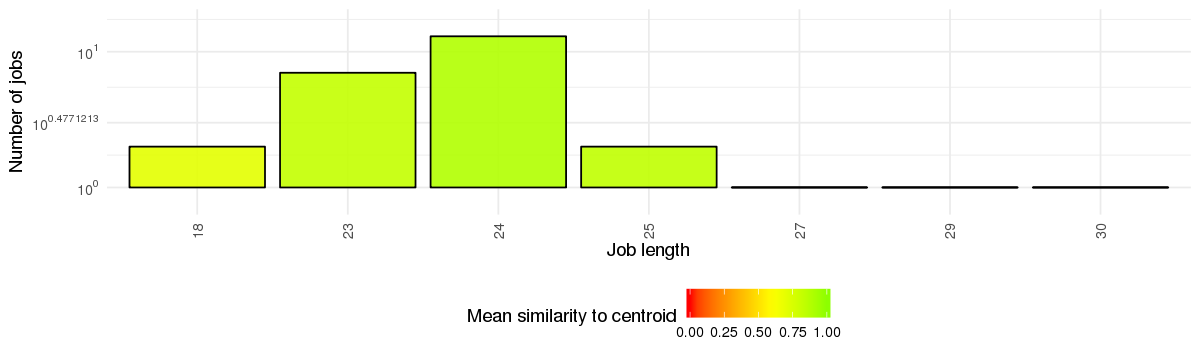
\includegraphics[width=4.61in,height=1.39in]{./media/image9.png}
  \captionof{figure}{Length distribution in the cluster.}
  \label{fig:use_case:bin_all:length}
\endgroup
%\end{figure}

\paragraph{BIN\_AGGZEROS}
Information related to the cluster is in \Cref{tab:use_case:bin_aggzeros:stats}, \Cref{tab:use_case:bin_aggzeros:top_jobs}, and in \Cref{fig:use_case:bin_aggzeros:length}.

%\begin{table}[h]
\begingroup
  \centering
  \begin{tabular}{ll}
    SIM & 0.7 \\
    Number of jobs & 8 \\
    Number of job types & 8 \\
  \end{tabular}
  \captionof{table}{Cluster statistics.}
  \label{tab:use_case:bin_aggzeros:stats}
\endgroup
%\end{table}

%\begin{table}[h]
\begingroup
  \centering
  \begin{tiny}
    \begin{tabular}{@{ }l@{ }|@{ }r@{ }}
      \rowcolor{tabhcolor}
      Binary coding                                                                                             &  Type     \\
      \hline
      192:192:192:192:192:192:196:192:192:192:192:192:192:192:192:192:192:192:192:192:192:192:64:64:64:64:64    &  job      \\
      511:238:192:510:192:224:228:192:192:192:192:192:192:192:192:192:192:192:192:192:192:64:64:64:64:64        &  centroid \\
      \multicolumn{2}{l}{}                                                                                      \\
      \rowcolor{tabhcolor}
      Binary coding                                                                                             &  Count    \\
      \hline
      0:224:192:192:192:192:228:192:192:192:192:192:192:192:192:192:192:192:192:192:192:64:64:64:64:64          &  1        \\
      192:192:192:192:192:192:196:192:192:192:192:192:192:192:192:192:192:192:192:192:192:192:64:64:64:64:64    &  1        \\
      192:192:193:196:192:192:192:192:192:192:192:192:192:192:192:192:192:192:192:192:64:64:64:64               &  1        \\
      192:193:193:198:192:192:192:192:192:192:192:192:192:192:192:192:192:192:192:192:192:64:64:64:64:64:64     &  1        \\
      207:463:225:495:246:224:198:192:192:192:192:192:192:192:192:192:192:192:192:192:192:192:64:64:64:64:64:64 &  1        \\
    \end{tabular}
  \end{tiny}
  \captionof{table}{Job, centroid and Top 5 job types.}
  \label{tab:use_case:bin_aggzeros:top_jobs}
\endgroup
%\end{table}

%\begin{figure}[h]
\begingroup
  \centering
  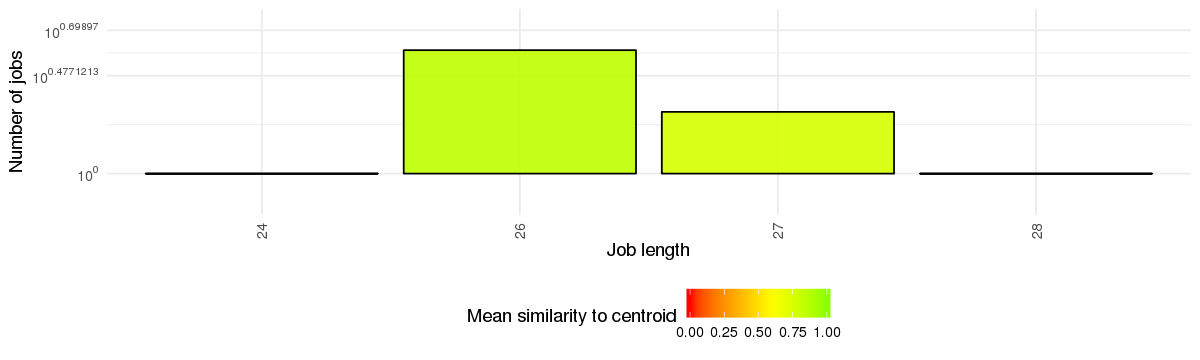
\includegraphics[width=4.61in,height=1.39in]{./media/image6.png}
  \captionof{figure}{Length distribution in the cluster.}
  \label{fig:use_case:bin_aggzeros:length}
\endgroup
%\end{figure}

\paragraph{HEX\_LEV}
Information related to the cluster is in \Cref{tab:use_case:hex_lev:stats}, \Cref{tab:use_case:hex_lev:top_jobs}, and in \Cref{fig:use_case:hex_lev:length}.

%\begin{table}[h]
\begingroup
  \centering
  \begin{tabular}{ll}
    SIM & 0.9 \\
    Number of jobs & 209 \\
    Number of job types & 189 \\
  \end{tabular}
  \captionof{table}{Cluster statistics.}
  \label{tab:use_case:hex_lev:stats}
\endgroup
%\end{table}

%\begin{table}[h]
\begingroup
  \begin{tiny}
    \begin{tabular}{@{ }l@{ }@{ }l@{ }|@{ }r@{ }}
      \rowcolor{tabhcolor}
      \multicolumn{2}{@{ }l|@{ }}{Hexadecimal coding} & \\
      \rowcolor{tabhcolor}
      md\_other                                           &  read\_calls                                           & Type     \\
      \hline
      0:\dots:0                                           &  3:3:8:8:8:5:6:8:8:8:8:8:8:8:8:8:8:8:8:8:8:8:8:8:8:8:8 & job      \\
      0:\dots:0                                           &  8:8:8:8:8:2:6:8:8:8:8:8:8:8:8:8:8:8:8:8:8:8:8:8:8:8:8 & centroid \\
      \multicolumn{3}{l}{}                                \\
      \rowcolor{tabhcolor}      md\_other                                           &  read\_calls                                           & Count    \\
      \hline
      0:\dots:0                                           &  0:0:0:0:0:0:8:8:8:8:8:8:8:8:8:8:8:8:8:8:8:8:8:8:8:8   & 4        \\
      0:\dots:0                                           &  8:8:8:8:8:2:8:8:8:8:8:8:8:8:8:8:8:8:8:8:8:8:8:8:8:8   & 4        \\
      0:0:0:4:0:0:0:0:0:0:0:0:0:0:0:0:0:0:0:0:0:0:0:0:0:0 &  0:0:0:0:0:0:8:8:8:8:8:8:8:8:8:8:8:8:8:8:8:8:8:8:8:8   & 4        \\
      0:\dots:0                                           &  8:8:8:8:8:3:8:8:8:8:8:8:8:8:8:8:8:8:8:8:8:8:8:8:8:8:8 & 3        \\
      0:\dots:0                                           &  0:0:0:0:0:0:2:8:8:8:8:8:8:8:8:8:8:8:8:8:8:8:8:8:8:8   & 2        \\
    \end{tabular}
  \end{tiny}
  \captionof{table}{Job, centroid and Top 5 job types.}
  \label{tab:use_case:hex_lev:top_jobs}
\endgroup
%\end{table}

%\begin{figure}[h]
\begingroup
  \centering
  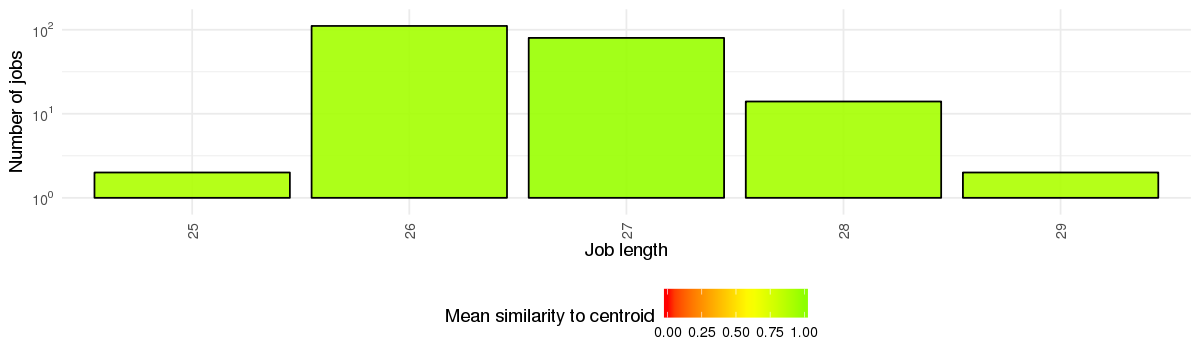
\includegraphics[width=4.61in,height=1.39in]{./media/image17.png}
  \captionof{figure}{Length distribution in the cluster.}
  \label{fig:use_case:hex_lev:length}
\endgroup
%\end{figure}

\paragraph{HEX\_NATIVE}
Information related to the cluster is in \Cref{tab:use_case:hex_native:stats}, \Cref{tab:use_case:hex_native:job_centroid}, and in \Cref{fig:use_case:hex_native:length}.

%\begin{table}[h]
\begingroup
  \centering
  \begin{tabular}{ll}
    SIM & 0.99 \\
    Number of jobs & 20 \\
    Number of job types & 20 \\
  \end{tabular}
  \captionof{table}{Cluster statistics.}
  \label{tab:use_case:hex_native:stats}
\endgroup
%\end{table}

%\begin{table}[h]
\begingroup
  \centering
  \begin{tiny}
    \begin{tabular}{@{ }l@{ }|@{ }r@{ }}
      \rowcolor{tabhcolor}
      Hexadecimal coding & \\
      \rowcolor{tabhcolor}
      read\_calls                                           & Type     \\
      \hline
      3:3:8:8:8:5:6:8:8:8:8:8:8:8:8:8:8:8:8:8:8:8:8:8:8:8:8 & job      \\
      8:8:8:8:8:2:4:8:8:8:8:8:8:8:8:8:8:8:8:8:8:8:8:8:8:8:8 & centroid \\
      \multicolumn{2}{l}{}\\
			\rowcolor{tabhcolor}
      read\_calls                                           & Count    \\
      \hline
      8:8:8:8:8:3:8:8:8:8:8:8:8:8:8:8:8:8:8:8:8:8:8:8:8:8:8 & 3        \\
      8:8:8:8:8:5:8:8:8:8:8:8:8:8:8:8:8:8:8:8:8:8:8:8:8:8:8 & 2        \\
      3:3:8:8:8:5:6:8:8:8:8:8:8:8:8:8:8:8:8:8:8:8:8:8:8:8:8 & 1        \\
      3:6:6:7:7:7:7:8:8:8:8:8:8:8:8:8:8:8:8:8:8:8:8:8:8:8:8 & 1        \\
      6:5:6:7:6:2:7:8:8:8:8:8:8:8:8:8:8:8:8:8:8:8:8:8:8:8:8 & 1        \\
    \end{tabular}
  \end{tiny}
  \captionof{table}{Job and centroid coding sequences.}
  \label{tab:use_case:hex_native:job_centroid}
\endgroup
%\end{table}

%\begin{figure}[h]\begingroup
\begingroup
  \centering
  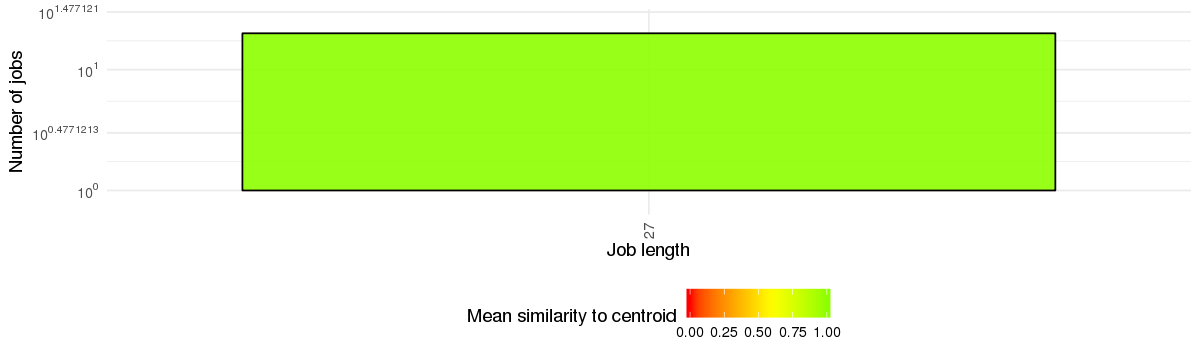
\includegraphics[width=4.61in,height=1.39in]{./media/image2.png}
  \captionof{figure}{Length distribution in the cluster.}
  \label{fig:use_case:hex_native:length}
\endgroup
%\end{figure}

\paragraph{PM\_QUANT}
Information\ related to the cluster is \Cref{tab:use_case:pm_quant:stats}, \Cref{tab:use_case:pm_quant:top_jobs}, and in \Cref{fig:use_case:pm_quant:length}.

%\begin{table}[h]
\begingroup
  \centering
  \begin{tabular}{ll}
    SIM                 & 0.7 \\
    Number of jobs      & 68  \\
    Number of job types & 59  \\
  \end{tabular}
  \captionof{table}{Cluster statistics.}
  \label{tab:use_case:pm_quant:stats}
\endgroup
%\end{table}

%\begin{table}[h]
\begingroup
  \centering
  \begin{tiny}
    \begin{tabular}{@{ }l@{ }|@{ }r@{ }}
      \rowcolor{tabhcolor}
      Hexadecimal coding & \\
      \rowcolor{tabhcolor}
      read\_calls                                           & Type     \\
      \hline
      3:3:8:8:8:5:6:8:8:8:8:8:8:8:8:8:8:8:8:8:8:8:8:8:8:8:8 & job      \\
      8:8:8:8:8:8:8:8:8:8:8:8:8:8:8:8:8:8:8:8:8:8:8:8:8:8   & centroid \\
      \multicolumn{2}{l}{}\\
      \rowcolor{tabhcolor}
      read\_calls                                           & Count    \\
      \hline
      8:8:8:8:8:2:8:8:8:8:8:8:8:8:8:8:8:8:8:8:8:8:8:8:8:8   & 4        \\
      8:8:8:8:8:3:8:8:8:8:8:8:8:8:8:8:8:8:8:8:8:8:8:8:8:8:8 & 3        \\
      7:7:7:7:7:2:8:8:8:8:8:8:8:8:8:8:8:8:8:8:8:8:8:8:8:8   & 2        \\
      8:8:8:8:8:5:8:8:8:8:8:8:8:8:8:8:8:8:8:8:8:8:8:8:8:8   & 2        \\
      8:8:8:8:8:8:8:8:8:8:8:8:8:8:8:8:8:8:8:8:8:8:8:8:8:8   & 2        \\
    \end{tabular}
  \end{tiny}
  \captionof{table}{Job, centroid and Top 5 job types.}
  \label{tab:use_case:pm_quant:top_jobs}
\endgroup
%\end{table}

%\begin{figure}[h]
\begingroup
  \centering
  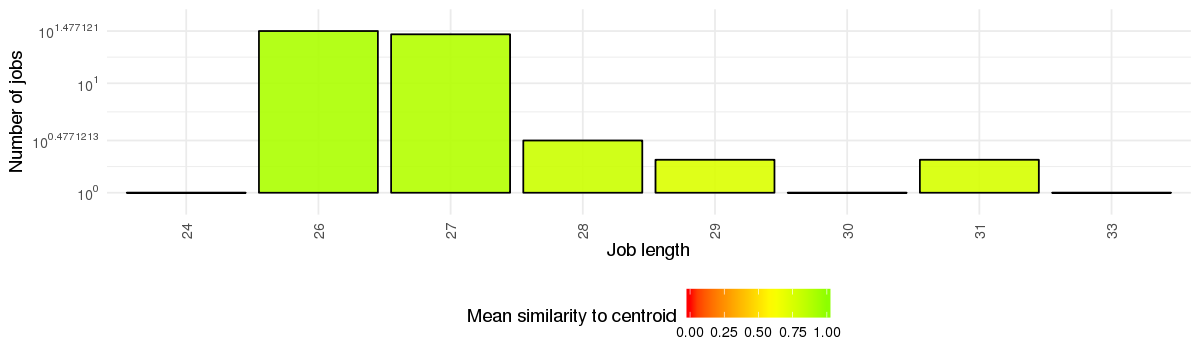
\includegraphics[width=4.61in,height=1.39in]{./media/image7.png}
  \captionof{figure}{Length distribution in the cluster.}
  \label{fig:use_case:pm_quant:length}
\endgroup
%\end{figure}

\subsubsection{Discussion}
Indeed clustering of hexadecimal codings produces usable results.
The examples in Table 2 show two randomly picked clusters.
The similar I/O behavior.

Another\ critical point of usage of Levenshtein distance is that it doesn't consider the performance.
For example, the following three codings would be considered as similar, since they differ in one position only.

\begin{lstlisting}
phase_coding_1 : [2:2:2:2:2:9:2:2]
phase_coding_2 : [2:2:2:2:2:8:2:2]
phase_coding_3 : [2:2:2:2:2:0:2:2]
\end{lstlisting}

Intuitively, we would say that {phase\_coding\_1 and{ phase\_coding\_2 are more similar than {phase\_coding\_2 and {phase\_coding\_3 , because the difference at 6th position is in the first case smaller (9 and 8) is smaller than in the second case (8 and 0).
Particularly bad affected are short coding, as the example in the previous sections shows.

The current version of the PM algorithm ignores non-IO parts (sequences of zeros) of the monitoring data, and  handles segment sequences like [0,0,0,0,1] and [1] equally.
These sequences would produce different average I/O loads on the storage.
Intuitively, we would say these jobs have different I/O behaviour and should consider that in the approach.


\begin{lstlisting}
job1_metric1 : [0,0,0,0,1]
job1_metric1 : [1]
\end{lstlisting}

One could also argue that the phase definition was chosen incorrectly.
Currently, phases are defined for each metric individually, without consideration what is going on on other metrics.
For illustration, consider the following two jobs.
Currently, the algorithm recognizes the I/O pattern as 100$\%$  similar.
Alternatively, one could say that running two metrics at the same time is another I/O pattern, as running them shifted, because on a storage system the jobs would produce different I/O loads.

\begin{lstlisting}
job1_metric1 : [0:1]
job1_metric2 : [1:0]
job2_metric1 : [1:0]
job2_metric2 : [1:0]
\end{lstlisting}

The benefit of ignoring these both aspects is simplicity.
This reduces the number of clusters and the results are easier to understand.
It also needs to be investigated, if these considerations are correct for HPC systems that are running hundreds of jobs in parallel, because one job alone would typically not be able to produce a significant amount of I/O that can slow down the file system performance.

The success of general purpose clustering and classification algorithms depends on right feature selection and data transformation.
In particular, feature selection is often quite challenging.
This makes training of models a kind of try and error approach.
Even if an optimal solution is found there is no guarantee that the approach with other data on other systems.

As you might have noticed, quantization is not necessary for PM.
It can perfectly work directly with floating point numbers, such as mean performance values.
The main motivation behind the use of hexadecimal coding is that it makes PM comparable with other algorithms.
For example, this allows us to see how the additional features affect the quality of clusters.
By accident, this was also the right decision.
We noticed that in the experiments with floating point numbers the amount of generated clusters skyrocketed.
The reason is that similarity for short jobs exceeds SIM value very fast and this leads to the creation of new clusters, which in turn leads to long clustering runtimes.
An example illustrates a typical case.
Assume there are two jobs: one running on 16 nodes and other running on 32 nodes.
Both are one segment long and only one I/O node that writes data to storage with a moderate performance.
Without quantization we would represent these jobs by the following sequences:  [..., [0.0625], $ \ldots $ ] and [..., [0.03125], ...], where only active metrics have values larger than zero.
Using the similarity function without quantization, i.e. with mean performance, would result in a similarity of 50$\%$ , and for SIM>0.5 they would be placed in separate clusters.
The hexadecimal coding filters these jobs automatically. Segments with mean performance less than 0.125 are quantized to zero and zero sequences are removed from the dataset. This problem doesn’t occur.
The main question remains what characterizes I/O and which characteristics should be involved in job comparison.

\begin{itemize}
	\item Are two jobs similar if they have similar I/O phases?
	\item Are two jobs similar if one job has an I/O phase at the beginning and the other at the same I/O phase at the end?
	\item Are two jobs similar if they have different lengths, but similar I/O phases?
\end{itemize}

To answer these questions we need a discussion with the community and a study of more use cases.
\subsection{Conclusion}
After a series of experiments with general purpose algorithms we could not achieve optimal results.
The investigation of resulting clusters shows that they are obviously polluted.
One problem might be that we apply a combination of a clustering and a classification algorithm.
The classification algorithm is trained by the potential erroneous output of the clustering algorithm and it can itself produce erroneous output, which multiples the total error.
Another problem might be that both algorithms are not aware of I/O performance and I/O phases.
As this work shows, this might be quite important.
At least, we achieve better results by considering both aspects.
The Levenshtein-distance based algorithms produce better, but still not sophisticated results.
This is a direct consequence of the usage of the Levenshtein distance, which is illustrated in the following example.
Suppose two jobs {[0:6:0:0]and [0:388:174:0] are in the same cluster with the centroid {[0:388:0:0].
Even if in both cases the similarity between the cluster and the centroid is 75$\%$  (only one change is required), we would intuitively say that these jobs are completely different, not even close to the 75$\%$  mark.
We can easily construct another sequence, e.g., {[0:389:0:0], where the 75$\%$  are justified.
The reason for such clustering failures, ist that Levenshtein distance is not able to extract and to use the meaning that was coded into the numbers.
Job comparison by means of hexadecimal coding is more precise, because hexadecimal coding sequences are much longer.
Absolute coding aggregates three dimensions (Metric, Nodes, and FileSystems) resulting in a nine times shorter coding sequence than hexadecimal coding, which aggregates only two dimensions (Nodes, and FileSystems).
Having more data, a more precise computation.
The integration of the awareness of I/O performance produces better, but still not sophisticated results.
We suppose that the I/O phase awareness is the missing feature for success.
The final algorithm that detects phases and differentiates performance values produces at first sight clean results.
Due to the huge amount of clusters and lack of automatic evaluation tools, we can not prove this statement for all clustres.
\subsection{Future work}
We see a high potential in the new clustering algorithm, but it requires some improvements to be useful.
Although groping seems to work well, the algorithm has at least one serious issue.
The biggest problem is probably the large number of clusters.
We assume that there indeed are so many different types of jobs, but there are too many of them for manual labeling.
Therefore we need at least three further functions, that filter irrelevant clusters, sort clusters by a criteria and label remaining ones.

%\setlength{\parskip}{0.0pt}
%\printbibliography
%\newpage
%\clearpage
%\pagebreak
\null
\bibliographystyle{splncs04}
\bibliography{bibliography}{}
\end{document}
